\documentclass[11pt]{article}

\usepackage[margin=1in]{geometry}
\usepackage{amsmath,amssymb}
\usepackage{graphicx}
\usepackage{xcolor}

\setlength{\parindent}{0pt}
\setlength{\parskip}{0.6em}

\begin{document}

\begin{center}
    {\Large\bfseries 2025 Final}
\end{center}

\vspace{1em}


\textbf{Q1. [20]} (A blast from the past. This question is from the materials right before the mid-term exam. Spatial connections in the space of distributions.)

Below we list ten(10) distributions (notations are as used in the class). Describe the inter-connections among all the distributions.

\textbf{(a)} Hypergeometric:
\[
\begin{aligned}
\Pr(X=x)&=\frac{\binom{r}{x}\binom{N-r}{n-x}}{\binom{N}{n}},\\
&\max(0,n-(N-r))\leq x\leq\min(r,n).
\end{aligned}
\]

\textbf{(b)} Binomial:
\[
\Pr(X=x)=\binom{n}{x}p^x(1-p)^{n-x},
\qquad x=0,1,2,\ldots,n.
\]

\textbf{(c)} Poisson:
\[
\Pr(X=x)=\frac{e^{-\lambda}\lambda^x}{x!},
\qquad x=0,1,2,\ldots
\]

\textbf{(d)} $N(0,1)$:
\[
f(x)=\frac{1}{\sqrt{2\pi}}e^{-x^2/2},
\qquad -\infty<x<\infty.
\]

\textbf{(e)} $N(\mu,\sigma^2)$:
\[
f(x)=\frac{1}{\sqrt{2\pi\sigma^2}}
\exp\left[-\frac{1}{2\sigma^2}(x-\mu)^2\right],
\qquad -\infty<x<\infty.
\]

\textbf{(f)} Gamma $(\alpha,\beta)$:
\[
f(x)=\frac{1}{\Gamma(\beta)\alpha^\beta}e^{-x/\alpha}x^{\beta-1},
\qquad 0<x<\infty.
\]

\textbf{(g)} Chi-squared, $\chi_n^2$ with $n$ d.f.:
\[
f(x)=\frac{1}{\Gamma(n/2)2^{n/2}}e^{-x/2}x^{\frac{n}{2}-1},
\qquad 0<x<\infty.
\]

\textbf{(h)} Student's $t$, $t_n$ (with $n$ d.f.):
\[
f(t)=\frac{\Gamma\left(\frac{n+1}{2}\right)}
{\sqrt{n\pi}\,\Gamma\left(\frac{n}{2}\right)}
\left(1+\frac{t^2}{n}\right)^{-\frac{n+1}{2}},
\qquad -\infty<t<\infty.
\]

\textbf{(i)} Cauchy:
\[
f(x)=\frac{1}{\pi}\frac{1}{1+x^2},
\qquad -\infty<x<\infty.
\]

\textbf{(j)} Pearson Type IV:
\[
f(x)=\text{const.}\,e^{-\left[\gamma\tan^{-1}(x/\alpha)\right]}
\left(1+\frac{x^2}{\alpha}\right)^{-m},
\qquad -\infty<x<\infty.
\]

\bigskip

\textbf{Q2. [2+8]} (Personalities from Probability and Statistics)

Pick any one from the following list. Write a couple of sentences on him/her. Then Write a short note on his/her contribution to the field of statistics.

\begin{enumerate}
    \item Thomas Bayes (1701--1761)
    \item Prasanta Chandra Mahalanobis (1893--1972)
    \item Friedrich Robert Helmert (1843--1917)
    \item Harald Cram\'er (1893--1985)
    \item Florence Nightingale David (1909--1993)
    \item Ronald A. Fisher (1890--1962)
    \item Karl Pearson (1857--1936)
    \item Andrei Kolmogorov (1903--1987)
    \item Corrado Gini (1884--1965)
    \item William S. Gosset (1876--1937)
\end{enumerate}

\bigskip

\textbf{Q3. [5+5+10+5+5]} \textbf{\textcolor{red}{Chapter 14}} (Estimating and Testing, Something Unnecessary!)

A smooth table (paper) is ruled with parallel lines at distance $a$ apart. A needle of length $\ell$ ($\ell<a$) is dropped randomly on the table (paper). The probability that the needle will cross one of the lines is
\[
P=\frac{2\ell}{a\pi}.
\]

\textbf{(a)} Now think about $\pi$, a Greek letter (thus not ``known'' to us). Using the above result, how can we estimate $\pi$?

\textbf{(b)} Is there any relationship between MLE and your estimator?

\textbf{(c)} Discuss unbiasedness, consistency, and efficiency of your estimator.

\textbf{(d)} Below is the outcome of dropping 30 needles (each of length 1/4 inch) randomly on this piece of paper, where parallel lines have been drawn at 1/3 inch apart. Using this experimental result, estimate the value of $\pi$.

\textit{Note:} 1 inch = 2.5 cm.

% Insert the figure from page 8 of the source PDF here.
% Put the image at images/2025_q3_needles.png; it will appear automatically.
\IfFileExists{images/2025_q3.png}{%
    \begin{center}
        
\includegraphics[width=0.75\textwidth]{images/2025_q3.png}
    \end{center}
}{}

\textbf{(e)} Is it possible to test $H_0:\pi=\frac{22}{7}$ using the available information? If so, how?

\bigskip

\textbf{Q4. [5+10+15]} \textbf{\textcolor{red}{Chapter 12}} (Remembering very old but useful friends, sample mean and sample variance)

\textbf{(a)} Let $X_i\overset{\mathrm{iid}}{\sim}N(\mu,\sigma^2)$, $i=1,2,\ldots,n$. Define
\[
\overline{X}=\frac{1}{n}\sum_{i=1}^n X_i,
\qquad
S^{\prime 2}=\frac{1}{n-1}\sum_{i=1}^n(X_i-\overline{X})^2.
\]
Write down the joint distribution of $\overline{X}$ and $S^{\prime 2}$ (no proof needed). Thus find $E(\overline{X})$, $\operatorname{Var}(\overline{X})$, $E(S^{\prime 2})$, $\operatorname{Var}(S^{\prime 2})$, and $\operatorname{Cov}(\overline{X},S^{\prime 2})$.

\textbf{(b)} Now relax the normality assumption, i.e. let $X_i\overset{\mathrm{iid}}{\sim}(\mu,\sigma^2)$, $i=1,\ldots,n$. Write down the joint distribution of $\overline{X}$ and $S^{\prime 2}$. Find $E(\overline{X})$, $\operatorname{Var}(\overline{X})$, and $E(S^{\prime 2})$. Show that
\[
\operatorname{Cov}(\overline{X},S^{\prime 2})=\frac{\mu_3}{n},
\]
where $\mu_3$ is the third central moment of $X$.

\textbf{(c)} Finally, find the asymptotic joint distribution of $\overline{X}$ and $S^{\prime 2}$, more specifically show that
\[
\sqrt{n}
\begin{pmatrix}
\overline{X}-\mu\\
S^{\prime 2}-\sigma^2
\end{pmatrix}
\overset{d}{\longrightarrow}
N\left(
\begin{pmatrix}0\\0\end{pmatrix},
\begin{pmatrix}
\sigma^2 & \mu_3\\
\mu_3 & \mu_4-\sigma^4
\end{pmatrix}
\right),
\]
where $\mu_4$ is the fourth central moment of $X$.

\textbf{Hint:} Recall that this problem is related to Q2 of Homework \#3. For this part, use the following result:
\[
\operatorname{Var}(S^{\prime 2})=
\frac{\mu_4}{n}-\frac{n-3}{n-1}\frac{\sigma^4}{n}.
\]

\bigskip

\textbf{Q5. [10]} \textbf{\textcolor{red}{Chapter 15}} (What happens when you Zzz.., while you should be drinking $t$ !)

Let $X_1,\ldots,X_n\overset{\mathrm{iid}}{\sim}N(\mu,\sigma^2)$ with unknown $\sigma^2$. The likelihood-ratio (LR) test for
\[
H_0:\mu=\mu_0\qquad\text{vs.}\qquad H_a:\mu\neq\mu_0
\]
is based on the statistic
\[
t=\frac{\sqrt{n}(\overline{X}-\mu_0)}{S'},
\]
which under $H_0$ has a $t_{n-1}$ distribution.

Discuss in detail what we will gain (or lose) if we use the normal ($Z$) table instead, to carry out the test, where
\[
Z=\frac{\sqrt{n}(\overline{X}-\mu_0)}{\sigma}.
\]

% ============================================================
% 2018 FINAL (append before \end{document})
% ============================================================
\clearpage

\begin{center}
    {\Large\bfseries 2018 Final}
\end{center}

\vspace{1em}

\textbf{Q1. [15 + 10 + 10]} \textbf{\textcolor{red}{Chapters 11}} (Let us start with an unusual way: By grading.)

\textbf{Part A:}

Below you are given a \textbf{Question} and a \textbf{Possible Answer}. Go over the Answer step-by-step and grade it, pointing out mistakes (if any) and praising clever steps (if any).

\textbf{Question:} Let $X_i\sim IIDN(\mu,\sigma^2)$, $i=1,2,\ldots,n$. Define
\[
\overline X=\frac{\sum_{i=1}^{n}X_i}{n}
\qquad\text{and}\qquad
S^2=\frac{1}{n}\sum_{i=1}^n(X_i-\overline X)^2.
\]
Show that $\dfrac{nS^2}{\sigma^2}\sim\chi^2_{n-1}$.

\textbf{Answer:} We can write
\[
\begin{aligned}
\sum_{i=1}^n(X_i-\overline X)^2
&=\sum_{i=1}^n\bigl[(X_i-\mu)-(\overline X-\mu)\bigr]^2\\
&=\sum_{i=1}^n(X_i-\mu)^2+n(\overline X-\mu)^2
   -2\sum_{i=1}^n(X_i-\mu)(\overline X-\mu)\\
&=\sum_{i=1}^n(X_i-\mu)^2+n(\overline X-\mu)^2,
\end{aligned}
\]
the last term being zero since $X_i$'s are independent.

Therefore,
\begin{equation}
\frac{nS^2}{\sigma^2}
=\sum_{i=1}^n\left(\frac{X_i-\mu}{\sigma}\right)^2
+\frac{n(\overline X-\mu)^2}{\sigma^2}.
\tag{1}
\end{equation}
Now
\[
\sum_{i=1}^n\left(\frac{X_i-\mu}{\sigma}\right)^2\sim\chi_n^2
\]
and
\[
\frac{n(\overline X-\mu)^2}{\sigma^2}
=\frac{(\overline X-\mu)^2}{\sigma^2/n}\sim\chi_1^2,
\qquad\text{since }\overline X\sim N\left(\mu,\frac{\sigma^2}{n}\right).
\]
Thus going back to the equation (1) above, we clearly see that
$\dfrac{nS^2}{\sigma^2}\sim\chi_{n-1}^2$. Q.E.D.

\textbf{Part B:}

Think of an alternative proof for the Question. And outline that Proof. Details are not necessary. Hint: Think of the Helmert transformation in the GPS (of your smartphone).

\textbf{Part C:}

Now relax the normality assumptions, i.e., $X_i\sim IID(\mu,\sigma^2)$, $i=1,2,\ldots,n$, and find the finite sample and asymptotic distributions of $S^2$.

\bigskip

\textbf{Q2. [10]} (Still unusual. A surprise visit.)

As your taking this test, suddenly you notice Karl Pearson (1857-1936) and Jerzy Neyman (1894-1981) walk into the Exam Hall DKH 123, and come directly to your desk. Then they have a 5-minute chat about their work covered in our Econ 532. Write down below your conversation with them.

\bigskip

\textbf{Q3. [10 + 5 + 5]} \textbf{\textcolor{red}{Chapter 15}} (Connecting Estimation and Testing.)

In the context of both estimation and testing we discussed the concepts of unbiasedness and consistency. Define those concepts and discuss their relationship(s) (if any).

What do we maximize (or minimize) in estimation and testing. What are the rational behind those optimizations?

Demonstrate (mathematically) the connections of sufficiency with the ideas of optimality in estimation and testing.

\bigskip

\textbf{Q4. [10 + 15]} \textbf{\textcolor{red}{Chapter 15}} (Mother and her children, and more...)

\textbf{(i)} State the fundamental principle of the Neyman-Pearson (NP) Lemma, the ``mother of all tests.'' Then from there find the basis of the likelihood ratio (LR) and Rao's score (RS) tests.

\textbf{(ii)} Suppose we want to test $H_0:\theta=\theta_0$ against $H_1:\theta\neq\theta_0$. Define and simplify the likelihood ratio (LR) (denoting it by $\lambda$) for testing $H_0$ vs. $H_1$.

Show (step-by-step) that under $H_0$:
\[
-2\log_e\lambda\overset{D}{\longrightarrow}\chi_1^2.
\]
[Hint: Use the following Taylor series expansion
\[
l(\theta_0)=l(\hat\theta)
+(\theta_0-\hat\theta)\left.\frac{\partial l(\theta)}{\partial\theta}\right|_{\hat\theta}
+\frac{1}{2}(\theta_0-\hat\theta)^2
 \left.\frac{\partial l^2(\theta)}{\partial\theta^2}\right|_{\theta^*},
\]
where $l(\theta)$ is the loglikelihood function, $\hat\theta$ is the MLE, and $\theta^*$ lies between $\theta_0$ and $\hat\theta$.] In your proof, you must mention \emph{all the results} that you use.

\bigskip

\textbf{Q5. [4 + 6]} \textbf{\textcolor{red}{Chapter 15}} (From your great experiment.)

Recall the grand experiment you conducted: Tossing a coin until you obtained two heads. Taking $X$ as the number of trials, in the table below probability mass function (pmf) of $X$ (in column 2), expected frequency (E) and observed frequency (O) are given. We also provide the $\chi^2$ goodness-of-fit statistic. The $\chi^2$ critical values (with 4 degrees of freedom) are 9.49 and 13.28, respectively, for significance level 0.05 and 0.01. Thus the null hypothesis is rejected.

\begin{center}
\small
\begin{tabular}{|c|c|c|c|}
\hline
$X$ & $\Pr(X=x)$ & Expected Frequency (E) & Observed Frequency (O)\\
\hline
2 & $1/4$ & 6 & 4\\ \hline
3 & $1/4$ & 6 & 4\\ \hline
4 & $3/16$ & 4.5 & 2\\ \hline
5 & $1/8$ & 3 & 5\\ \hline
6 or more & $3/16$ & 4.5 & 9\\ \hline
Total & 1 & 24 & 24\\ \hline
\end{tabular}
\end{center}

\[
\begin{aligned}
\chi^2&=\sum_{j=1}^{5}\frac{(E_j-O_j)^2}{E_j}\\
&=\frac{(6-4)^2}{6}+\frac{(6-4)^2}{6}
+\frac{(4.5-2)^2}{4.5}+\frac{(3-5)^2}{3}
+\frac{(4.5-9)^2}{4.5}\approx19.67
\end{aligned}
\]

\textbf{(i)} What is the null hypothesis here?

\textbf{(ii)} Suppose all of you have used the \textbf{same} coin to conduct the experiment. Given the data (the observed frequencies), can you say something about the value(s) of $P(H)$ of the coin? (Hint: Think about what value(s) of p=Probability of Head=P(H) could have led to the observed data.)












% ============================================================
% 2017 FINAL (append before \end{document})
% ============================================================
\clearpage

\begin{center}
    {\Large\bfseries 2017 Final}
\end{center}

\vspace{1em}

\textbf{Q1. [15 + 10]} \textbf{\textcolor{red}{Chapter 9}} (Let us start with business as normal)

\textbf{(i)} Express $\overline X=\sum_{i=1}^{n}X_i/n$ and $S^2=\sum_{i=1}^{n}(X_i-\overline X)^2/n$, respectively, as a linear and quadratic forms of the $(n\times 1)$ vector $\underset{\sim}{X}=(X_1,X_2,\ldots,X_n)'$.

\textbf{(ii)} Using the results of (i), show that $\overline X$ and $S^2$ are independently distributed. To answer this question, make assumption(s) as needed.

\bigskip

\textbf{Q2. [5 + 10]} \textbf{\textcolor{red}{Chapter 10}} (Asymptotics)

\textbf{(i)} Show that $t_n\overset{p}{\longrightarrow} Z$, where $Z\sim N(0,1)$.

\textbf{(ii)} Demonstrate how $B(n,p)$ and $\chi_n^2$ converge in distribution to $N(0,1)$. Make assumptions (and adjustments) as needed.

\bigskip

\textbf{Q3. [25 + 5]} \textbf{\textcolor{red}{Chapter 14}} (Some theory)

\textbf{(i)} Consider the MLE of $\theta$, $\hat\theta$. Using the result that $\hat\theta\overset{p}{\longrightarrow}\theta$, show
\[
\sqrt{n}(\hat\theta-\theta)\overset{D}{\longrightarrow}N\left(0,1/\nu(\theta)\right),
\]
where
\[
\nu(\theta)=E\left[\frac{d\log f(x,\theta)}{d\theta}\right]^2
=E\left[-\frac{d^2\log f(x,\theta)}{d\theta^2}\right].
\]
In your proof you must state all the assumptions, and results you use. [Hint: Use the following Taylor series expansion:
\[
0=\left.\frac{1}{n}\frac{dl(\theta)}{d\theta}\right|_{\hat\theta}
=\frac{1}{n}\frac{dl(\theta)}{d\theta}
+\left.\frac{1}{n}\frac{d^2 l(\theta)}{d\theta^2}\right|_{\theta^*}(\hat\theta-\theta),
\]
where $l(\theta)$ is the log-likelihood function and $\theta^*$ lies between the true value $\theta$ and $\hat\theta$].

\textbf{(ii)} Interpret the result in (i) in terms of efficiency of $\hat\theta$.

\bigskip

\textbf{Q4. [5 + 5 + 15]} \textbf{\textcolor{red}{Chapter 15}} (On God's result: Neyman-Pearson Theory)

\textbf{(i)} Look at the cartoons again on the coverage and consider the definitions of Type-I and Type-II errors. Are the two figures properly classified? If not, why not?

% The original exam places the two cartoons on the cover (PDF page 1),
% with the caption: H_0: Pregnant, H_a: Not pregnant.
% Save a crop of those cartoons as images/2017_q4_cartoons.png.
% The image will appear automatically once the file is available.
\IfFileExists{images/2017_q4_cartoons.png}{%
    \begin{center}
      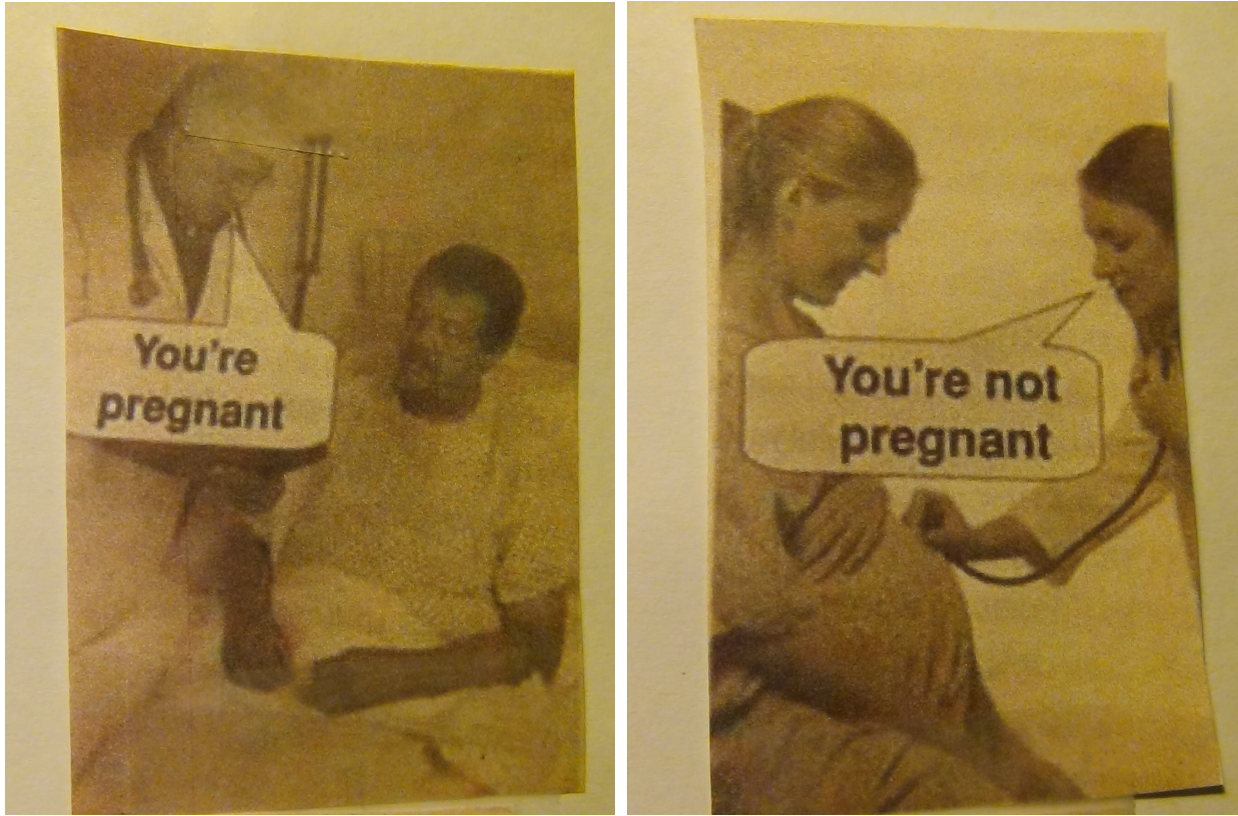
\includegraphics[width=0.78\textwidth]{images/2017_q4_cartoons.png}
    \end{center}
}{}

\textbf{(ii)} We defined an unbiased critical region (or test) $\omega$ for testing $H_0:\theta=\theta_0$ against $H_a:\theta\neq\theta_0$ if $\Pr(W\in\omega\mid H_0)=\alpha$ and $\Pr(W\in\omega\mid H_a)\geq\alpha$, where $W$ is the test statistic. On the other hand we defined an estimator $\hat\theta$ to be \emph{unbiased} if $E(\hat\theta)=\theta$. Connect these two definitions of unbiasedness.

\textbf{(iii)} Recall what we said in class: ``Neyman-Pearson Lemma is the mother of `all' tests.'' Justify this statement for the likelihood ratio (LR) and the Rao Score (RS) test.

\clearpage

\textbf{Q5. [5 + 5]} (Personalities in Statistics)

Write short (really short) notes on any \textbf{two} of the following personalities relating them to our ECON 532:

\textbf{(a)} Ireneo Funes in the short story of Jorge Luis Borges (1899-1986).

\textbf{(b)} Pearson (1895-1980).

\textbf{(c)} Prasanta Chandra Mahalanobis (1893-1972).

\bigskip

\textbf{Finally, Q6.} (Reliability of This Exam)

As we discussed in class, in psychometry there is a concept of Reliability which is the degree to which an assessment tool (like this Exam) produces stable and consistent result. In your view, what is the reliability of this Final Exam. Write down below on the line, on a scale 0 (worst) to 100 (best):

Score: \underline{\hspace{5cm}}


% ============================================================
% 2016 FINAL (append before \end{document})
% ============================================================
\clearpage

\begin{center}
    {\Large\bfseries 2016 Final}
\end{center}

\vspace{1em}

\textbf{Q1. [10]} \textbf{\textcolor{red}{Chapter 15}} (Looking back)

Recall you (the Econ 532 class, Fall 2016) reported the number of trials ($X$) needed to obtain the first head by tossing ``unbiased'' coins. A summary of your data is given below:

\begin{center}
\begin{tabular}{lr}
\hline
Value of $X$ & Observed Frequency \\
\hline
1 & 14 \\
2 & 10 \\
3 & 6 \\
4 & 5 \\
5 or more & 5 \\
Total & 40 \\
\hline
\end{tabular}
\end{center}

Given these results what would be a ``nice'' hypothesis to test? State your null and alternative hypotheses and carry out an appropriate test.

Hint: You may use the following Pearson $\chi^2$-test statistic:
\[
\chi_P^2=\sum_{j=1}^{r}\frac{(E_j-O_j)^2}{E_j},
\]
which approximately follows an $\chi^2_{r-1}$, where $E_j$ and $O_j$ are, respectively, the expected and observed frequencies, and $r$ is the number of classes or groups. $\chi^2_{0.05,5}=11.070$, and $\chi^2_{0.05,4}=9.488$.

\bigskip

\textbf{Q2. [5 + 10 + 5]} \textbf{\textcolor{red}{Chapter 15}} (The Great Expectations)

A table of your expected midterm (Fall 2016) grade ($X$), observed grade ($Y$) (along with the scatter plot), and the difference ($Z=X-Y$) as reported by thirty eight (38) students is given in the next page. Here the numbers 1, 2, 3, 4, 5, 6, 7, 8 and 9 correspond to letter grades $C-$, $C$, $C+$, $B-$, $B$, $B+$, $A-$, $A$ and $A+$, respectively.

\textbf{(i)} Discuss their differences between $(\overline X, S_X^{\prime 2})$ and $(\overline Y, S_Y^{\prime 2})$, if any.

\textbf{(ii)} Now we want to test $H_0:\mu_X=\mu_Y$. Write down your test procedure, and interpret the result.

\textbf{(iii)} Now think about dividing the students in top 50\% and the rest, and testing the same hypothesis $H_0:\mu_X=\mu_Y$ separately, for these two groups. What would you expect? Discuss your answer without doing any explicit calculations.

\begin{center}
{\small
\setlength{\tabcolsep}{9pt}
\renewcommand{\arraystretch}{0.91}
\begin{tabular}{lrrr}
\hline
 & $X$ & $Y$ & $Z$ \\
\hline
 & 9 & 9 & 0 \\
 & 9 & 6 & 3 \\
 & 9 & 7 & 2 \\
 & 9 & 8 & 1 \\
 & 9 & 7 & 2 \\
 & 8 & 7 & 1 \\
 & 8 & 9 & -1 \\
 & 8 & 9 & -1 \\
 & 8 & 5 & 3 \\
 & 8 & 8 & 0 \\
 & 7 & 6 & 1 \\
 & 7 & 9 & -2 \\
 & 7 & 8 & -1 \\
 & 7 & 8 & -1 \\
 & 7 & 4 & 3 \\
 & 7 & 3 & 4 \\
 & 6 & 8 & -2 \\
 & 6 & 6 & 0 \\
 & 6 & 6 & 0 \\
 & 6 & 6 & 0 \\
 & 6 & 6 & 0 \\
 & 6 & 6 & 0 \\
 & 5 & 3 & 2 \\
 & 5 & 5 & 0 \\
 & 5 & 7 & -2 \\
 & 5 & 5 & 0 \\
 & 5 & 6 & -1 \\
 & 4 & 8 & -4 \\
 & 4 & 7 & -3 \\
 & 4 & 2 & 2 \\
 & 4 & 7 & -3 \\
 & 3 & 5 & -2 \\
 & 3 & 3 & 0 \\
 & 3 & 6 & -3 \\
 & 2 & 5 & -3 \\
 & 2 & 3 & -1 \\
 & 2 & 3 & -1 \\
 & 1 & 2 & -1 \\
\hline
Mean & 5.79 & 6.01 & $-0.21$ \\
Variance & 5.14 & 4.11 & 3.68 \\
\hline
\end{tabular}
}
\end{center}

% The original source contains a scatter plot beside the data table
% on PDF page 4. Save just the graph as images/2016_q2_scatter.png.
% It will be included automatically when the image is available.
\IfFileExists{images/2016_q2.png}{%
    \begin{center}
      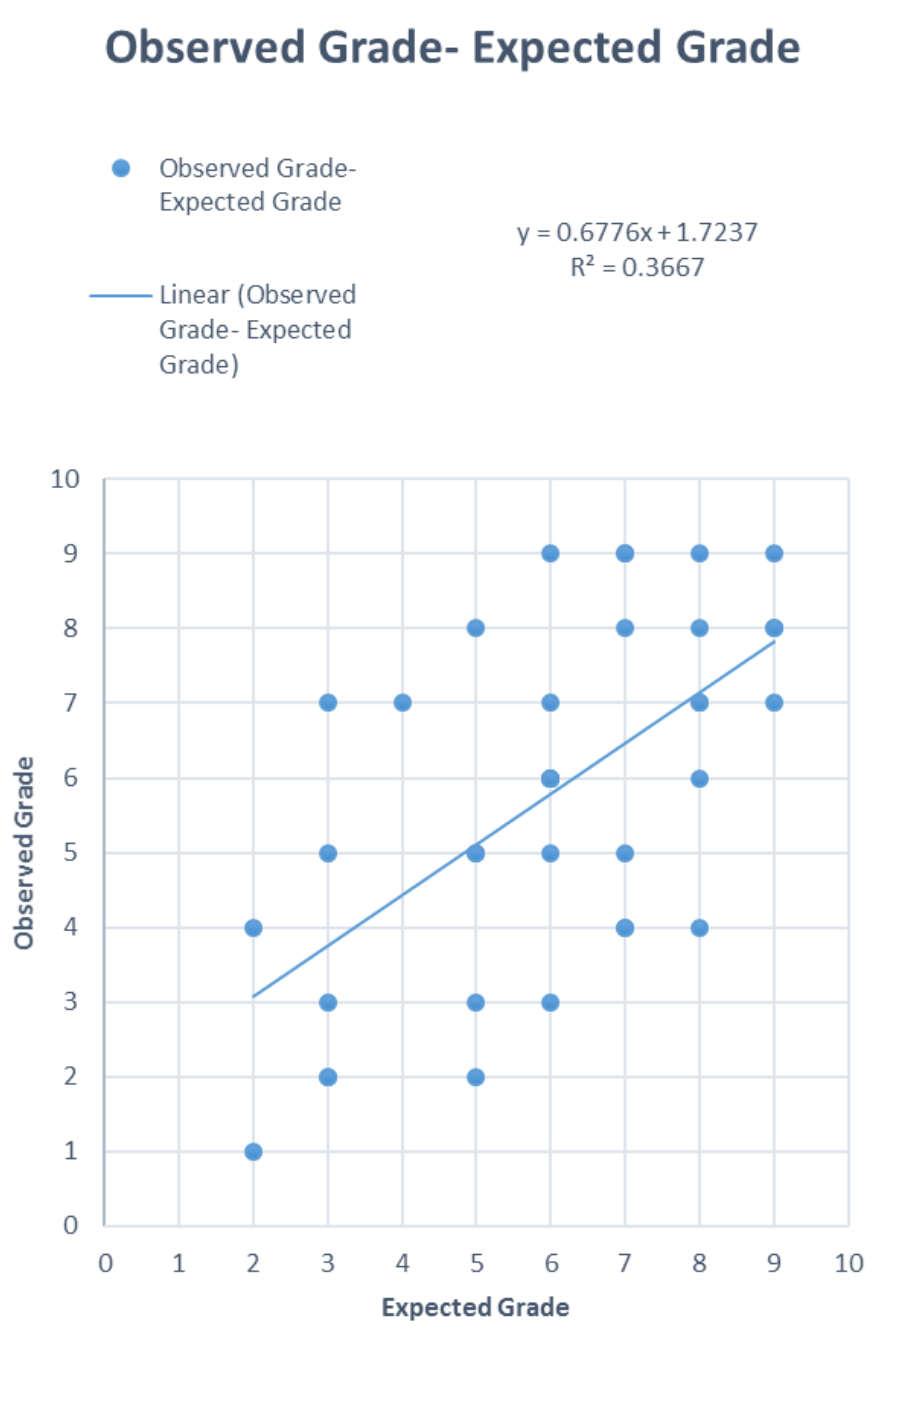
\includegraphics[width=0.68\textwidth]{images/2016_q2.png}
    \end{center}
}{}

Formula used, for example,

Sample mean:
\[
\overline X=\sum_{i=1}^{n}X_i/n.
\]
Sample Variance:
\[
S_X^{\prime 2}=\sum_{i=1}^{n}(X_i-\overline X)^2/(n-1).
\]

\clearpage

\textbf{Q3. [15 + 10]} \textbf{\textcolor{red}{Chapters 10 and 13}} (Asymptotics)

\textbf{(i)} If $g(\cdot)$ is a continuous function on the real line and $X_n\overset{p}{\longrightarrow}X$, then show that $g(X_n)\overset{p}{\longrightarrow}g(X)$.

Hint: Use continuity of $g(\cdot)$: For a given $\epsilon>0$, there exists a $\delta>0$ such that $|x_n-x|\leq\delta\Rightarrow |g(X_n)-g(X)|<\epsilon$.

\textbf{(ii)} Using central limit theorem (CLT), show that
\[
\frac{\chi_n^2-n}{\sqrt{2n}}\overset{D}{\longrightarrow}N(0,1).
\]

\bigskip

\textbf{Q4. [25 + 5]} \textbf{\textcolor{red}{Chapter 14}}  (Some theory)

\textbf{(i)} Consider the MLE of $\theta$, $\hat\theta$. Using the result that $\hat\theta\overset{p}{\longrightarrow}\theta$, show
\[
\sqrt{n}(\hat\theta-\theta)\overset{D}{\longrightarrow}N\left(0,1/\nu(\theta)\right),
\]
where
\[
\nu(\theta)=E\left[\frac{d\log f(x,\theta)}{d\theta}\right]^2
=E\left[-\frac{d^2\log f(x,\theta)}{d\theta^2}\right].
\]
In your proof you must state all the assumptions, and results you use. [Hint: Use the following Taylor series expansion:
\[
0=\left.\frac{1}{n}\frac{dl(\theta)}{d\theta}\right|_{\hat\theta}
=\frac{1}{n}\frac{dl(\theta)}{d\theta}
+\left.\frac{1}{n}\frac{d^2l(\theta)}{d\theta^2}\right|_{\theta^*}(\hat\theta-\theta),
\]
where $l(\theta)$ is the log-likelihood function and $\theta^*$ lies between the true value $\theta$ and $\hat\theta$].

\textbf{(ii)} Interpret the result in (i) in terms of efficiency of $\hat\theta$.

\clearpage

\textbf{Q5. [15]} \textbf{\textcolor{red}{Chapter 15}} (Testing/Tasting)

Prove the Neyman-Pearson Lemma as given below:

A critical region $\omega_0$ of size $\alpha$ is most powerful if inside $\omega_0$,
\[
\frac{L(\theta_0)}{L(\theta_a)}<k,
\]
and outside $\omega_0$,
\[
\frac{L(\theta_0)}{L(\theta_a)}\geq k,
\]
where $k$ is such that $\Pr\left(\left.\frac{L(\theta_0)}{L(\theta_a)}<k\,\right|H_0\right)=\alpha$.

Notations are as used in the class. However, you should explain the notations, and introduce new ones as needed and state the required assumptions.

\bigskip

\textbf{Q6. [5 + 5]} (Some Leading Personalities in Statistics who Influenced our Econ 532)

Write a short note (between the two-lines below) on the life and work of any one of the following personalities:

Karl Pearson

Prasanta Chandra Mahalanobis

Jerzy Neyman

David Blackwell

Calyampudi Radhakrishna Rao


% ============================================================
% 2015 FINAL (append before \end{document})
% ============================================================
\clearpage

\begin{center}
    {\Large\bfseries 2015 Final}
\end{center}

\vspace{1em}

\textbf{Q1. [10 + 5]} (A helicopter tour of estimation and testing)

\textbf{(i)} Summarize what you have learned in the second part of the course, i.e., on estimation and testing. Write your answer in the space provided (i.e., between the two lines).

\textbf{(ii)} (Movie) Recall that the Tollywood (made in Tollygunge, Calcutta) movie, that we watched last week in class, on Professor Prasanta Chandra Mahalanobis. He talked about Statistics as a Technology. Is it possible to view our second part of course as ``technology''? Justify your answer. Again, write in the space provided.

\bigskip

\textbf{Q2. [8 + 12 + 10]} \textbf{\textcolor{red}{Chapters 9 and 15}} (Some theory)

Given a random sample $\{X_1,X_2,\ldots,X_n\}$ from the population $N(\mu,\sigma^2)$, define
\[
\overline X=\frac{\sum_{i=1}^{n}X_i}{n},\qquad
S^2=\frac{1}{n}\sum_{i=1}^{n}(X_i-\overline X)^2,
\]
\[
S^{\prime 2}=\frac{1}{n-1}\sum_{i=1}^{n}(X_i-\overline X)^2
\quad\text{and}\quad
S_0^2=\frac{1}{n}\sum_{i=1}^{n}(X_i-\mu)^2.
\]

In the class, we proved that $\overline X$ and $S^2$ are independent, and they are distributed as, respectively,
\[
\overline X\sim N\!\left(\mu,\frac{\sigma^2}{n}\right)
\quad\text{and}\quad
\frac{nS^2}{\sigma^2}\sim\chi^2_{n-1}.
\]

\textbf{(i)} Using the \emph{above} results, find the distribution of $\dfrac{nS_0^2}{\sigma^2}$. Then compare the variance of $S^2$ and $S_0^2$ and explain your result.

\textbf{(ii)} State the distributions of the following statistics (\emph{derivations are not required}):
\[
\frac{\sqrt n\,\overline X}{\sigma},\qquad
\frac{\sqrt n(\overline X-\mu)}{S},\qquad
\frac{\sqrt{n-1}(\overline X-\mu)}{S'},\qquad
\frac{\sqrt n(\overline X-\mu)}{S'}.
\]

\textbf{(iii)} Suppose we want to test $H_0:\mu=0$ against $H_a:\mu\neq 0$. The likelihood ratio (LR) test for this problem, with size $\alpha$, is to reject $H_0$ if
\[
\left|\frac{\sqrt n\,\overline X}{S'}\right|>t_{\alpha/2,n-1}.
\]
Discuss the consequences of using the standard normal distribution table (Z-table) in carrying out this test. Under what circumstance(s), use of Z-table can be justified?

\bigskip

\textbf{Q3. [5 + 10 + 10]} \textbf{\textcolor{red}{Chapter 15}} (Manpower or womanpower?)

I separated your mid-term grades (expected and observed) for two groups: Male and Female students, denoted by $X$ and $Y$, respectively.

\textbf{(i)} Discuss the dependence between $X$ and $Y$ (both expected and observed cases).

\textbf{(ii)} Below are empirical density plots. Discuss the differences/similarities between the plots for male and female in Figure 1 and Figure 2 (separately).

\textbf{Density plots for male and female}

For expected grades:

% Original exam, PDF page 6: Figure 1 (kernel density of expected grades).
% Save the cropped graph as images/2015_q3_expected.png.
\IfFileExists{images/2015_q3_expected.png}{%
    \begin{center}
      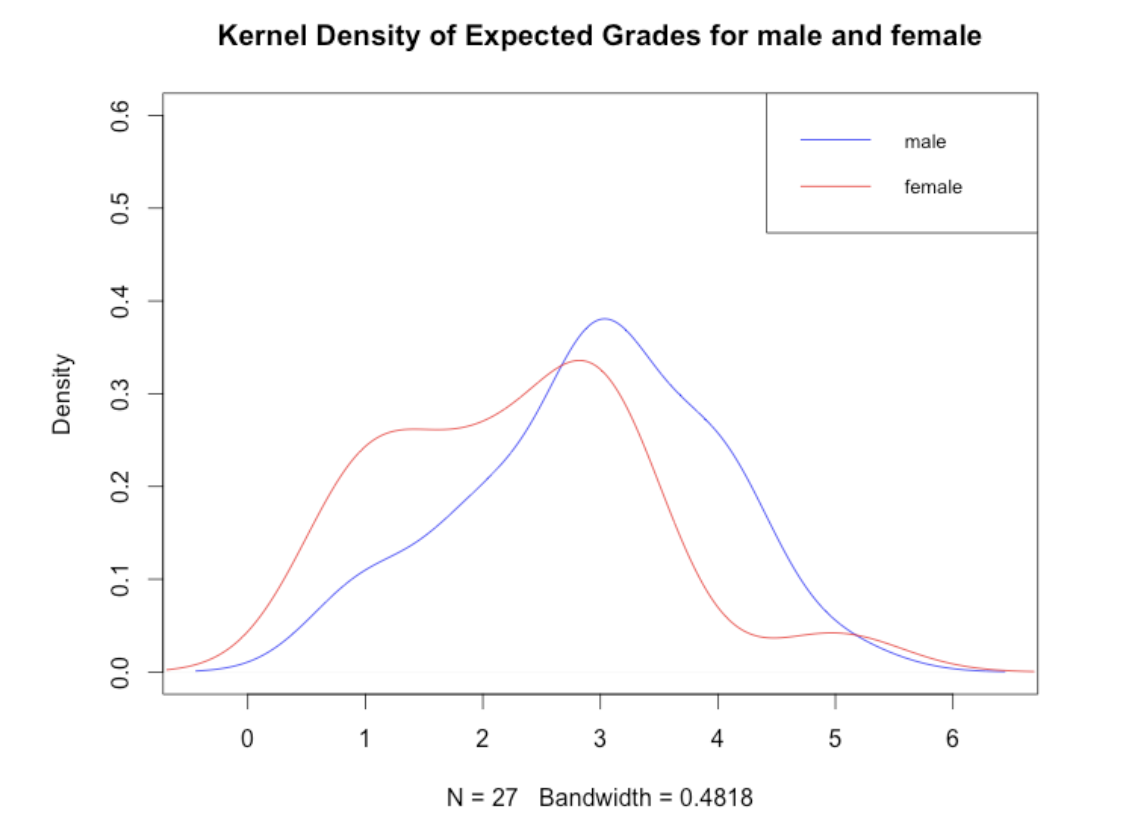
\includegraphics[width=0.74\textwidth]{images/2015_q3_expected.png}\\
      Figure 1
    \end{center}
}{}

For observed grades:

% Original exam, PDF page 6: Figure 2 (kernel density of observed grades).
% Save the cropped graph as images/2015_q3_observed.png.
\IfFileExists{images/2015_q3_observed.png}{%
    \begin{center}
      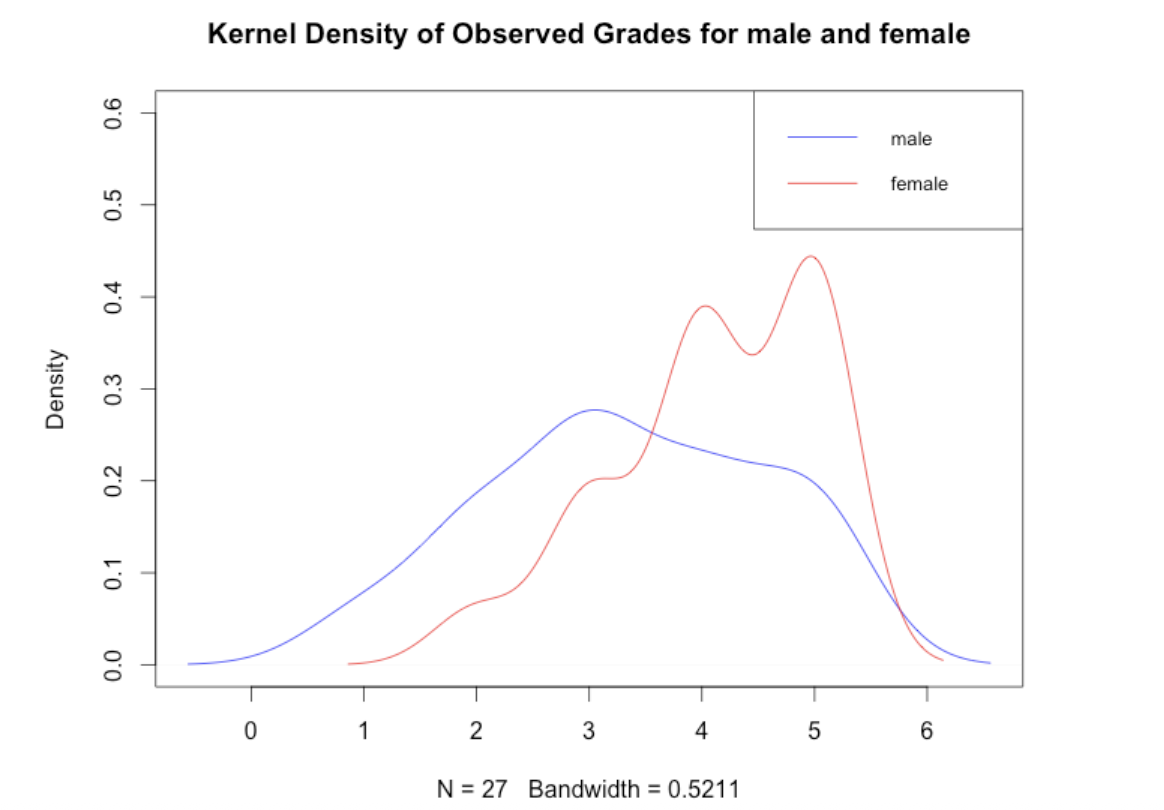
\includegraphics[width=0.74\textwidth]{images/2015_q3_observed.png}\\
      Figure-2
    \end{center}
}{}

\textbf{(iii)} The expected and observed scores for 27 ($n_1$) male and 17 ($n_2$) female students are given below:

\emph{Expected grades}

Male: 2,2,4,3,3,2,2,3,1,3,3,4,4,5,3,4,4,1,1,3,4,3,3,3,3,2,4

Female: 2,3,3,1,3,1,3,2,2,5,3,1,3,2,3,1,1

\emph{Observed grades}

Male: 4,3,5,3,2,2,3,3,1,3,5,3,5,4,4,4,5,2,2,5,5,4,1,4,3,2,3

Female: 5,4,5,4,5,3,4,4,3,5,5,5,5,3,4,4,2

The numbers 1,2,3,4,5 correspond to grades $B$, $B^+$, $A^-$, $A$, $A^+$, respectively.

Using these we can calculate the sample mean and variances as follows:

\begin{center}
\begin{tabular}{lcccc}
\hline
 & \multicolumn{2}{c}{Expected grades} & \multicolumn{2}{c}{Observed grades}\\
 & Mean & Variance & Mean & Variance\\
\hline
Male ($X$) & 2.92 & 1.07 & 3.33 & 1.53\\
Female ($Y$) & 2.29 & 1.22 & 4.12 & 0.86\\
\hline
\end{tabular}
\end{center}

Test the hypothesis $H_0:\mu_x=\mu_y$, both for the expected and observed grades. For carrying out the tests you formulate the appropriate alternative hypotheses.

Hint: Use
\[
t=\frac{\overline X-\overline Y}{\left[\frac{(n_1-1)S_x^{\prime 2}+(n_2-1)S_y^{\prime 2}}{n_1+n_2-2}\left(\frac{1}{n_1}+\frac{1}{n_2}\right)\right]^{1/2}}.
\]

\bigskip

\textbf{Q4. [10]} \textbf{\textcolor{red}{Chapter 10}} (A little more theory)

Consider
\[
t=\frac{\sqrt n\,(\overline X-\mu)}{S'},
\]
where $X_i\sim\mathrm{IID}(\mu,\sigma^2)$, $i=1,2,\ldots,n$, $\overline X=\sum_{i=1}^{n}X_i/n$, $S^{\prime 2}=\sum_{i=1}^{n}(X_i-\overline X)^2/(n-1)$.

Show that
\[
t\overset{D}{\longrightarrow}N(0,1).
\]

Hint: Use both law of large numbers and central limit theorem.

\bigskip

\textbf{Q5. [15 + 5]} \textbf{\textcolor{red}{Chapter 14}} (Yet more theory)

\textbf{(i)} Consider the MLE of $\theta$, $\hat\theta$. Using the result that $\hat\theta\overset{p}{\longrightarrow}\theta$, show
\[
\sqrt n(\hat\theta-\theta)\overset{D}{\longrightarrow}N\!\left(0,1/\nu(\theta)\right),
\]
where
\[
\nu(\theta)=E\left[\frac{d\log f(x,\theta)}{d\theta}\right]^2
=E\left[-\frac{d^2\log f(x,\theta)}{d\theta^2}\right].
\]

In your proof you must state all the assumptions, and results you use. [Hint: Use the following Taylor series expansion:
\[
0=\left.\frac{1}{n}\frac{dl(\theta)}{d\theta}\right|_{\hat\theta}
=\frac{1}{n}\frac{dl(\theta)}{d\theta}
+\left.\frac{1}{n}\frac{d^2l(\theta)}{d\theta^2}\right|_{\theta^*}(\hat\theta-\theta),
\]
where $l(\theta)$ is the log-likelihood function and $\theta^*$ lies between the true value $\theta$ and $\hat\theta$].

\textbf{(ii)} Interpret the result in (i) in terms of efficiency of $\hat\theta$.

\bigskip

\textbf{Q6. [5 + 5]} \textbf{\textcolor{red}{Chapter 13}} (Sufficiency is sufficient)

Proof that if there is a sufficient statistic $T$ for the parameter $\theta$, then both the most powerful (MP) test statistic (for $\theta$) and the maximum likelihood estimator (MLE) of $\theta$ are functions of $T$.


% ============================================================
% 2014 FINAL (append before \end{document})
% ============================================================
\clearpage

\begin{center}
    {\Large\bfseries 2014 Final}
\end{center}

\vspace{1em}

\textbf{Q1. [5]} (Prologue: The Fundamental Question)

What is Statistics? [Hint: Use maximum five sentences to answer this].

\bigskip

\textbf{Q2. [10 + 15 + 5]} \textbf{\textcolor{red}{Chapter 9}} (Our Old Friends: Mean and Variance)

\textbf{(i)} Let $X_i\sim\mathrm{IIDN}(\mu,\sigma^2)$, $i=1,2,\ldots,n$.

Define
\[
\overline X=\frac{\sum_{i=1}^{n}X_i}{n}
\qquad\text{and}\qquad
S^{\prime 2}=\frac{\sum_{i=1}^{n}(X_i-\overline X)^2}{n-1}.
\]
Find $E(\overline X)$, $E(S^{\prime 2})$, $Var(\overline X)$, and $Var(S^{\prime 2})$.

\textbf{(ii)} Now relax the independence assumption: Let $Corr(X_i,X_j)=\rho>0$, $i\neq j$. Now find $E(\overline X)$, $E(S^{\prime 2})$ and $Var(\overline X)$.

\textbf{(iii)} Interpret the differences (if any) in the expressions of $Var(\overline X)$ in (i) and (ii).

\bigskip

\textbf{Q3. [10]} \textbf{\textcolor{red}{Chapter 10}} (A Little Theory)

Let $Y\sim\chi_n^2$. Using the Lindeberg-Levy central limit theorem show that
\[
\frac{Y-n}{\sqrt{2n}}\overset{D}{\longrightarrow}N(0,1).
\]

[Lindeberg-Levy central limit theorem: Let $X_i\sim\mathrm{IID}(\mu,\sigma^2)$, $i=1,2,\ldots,n$, $0<\sigma^2<\infty$. Then
$\dfrac{\overline X_n-\mu}{\sigma/\sqrt n}\overset{D}{\longrightarrow}N(0,1)$, where $\overline X_n=\dfrac{1}{n}\sum_{i=1}^{n}X_i$.]

\bigskip

\textbf{Q4. [10 + 5 + 10]} \textbf{\textcolor{red}{Chapter 14}} (Stats on Rats)

Read the attached \emph{New York Times}, November 5th article. Estimating the number of rats (say, $\theta$) is indeed an important exercise. I also have rat problem in my house. To estimate the number of rats, I used the ``capture-recapture method'' (discussed in class). First, I caught $r=9$ rats, marked and released (I did not need city-permission for that) them. My second sample consisted of $n=8$ rats, of which I found, $X=4$ are marked.

\textbf{(i)} Estimate the number of rats in my house. [Hint: you must write the algebraic expression of your estimator, $\hat\theta$ (with derivation, if needed)].

\textbf{(ii)} Compare the ``capture-recapture'' method with that of Mr. Auerbach, mentioned in the \emph{New York Times} article.

\textbf{(iii)} Is $\hat\theta$ in (i) an ML, MM, or minimum $\chi^2$ or some other estimator? Show that $E(X)=\dfrac{nr}{\theta}$. What does this imply? [Hint: Think in terms of Binomial distribution with a ``large'' $\theta$].

% Attached New York Times article: source PDF pages 15--17.
% Save the three article pages as follows if you wish to insert them:
% images/2014_q4_article_1.png, images/2014_q4_article_2.png,
% images/2014_q4_article_3.png.
% The optional figures below will appear only if the files exist.
\IfFileExists{images/2014_q4_article_1.png}{%
    \begin{center}
    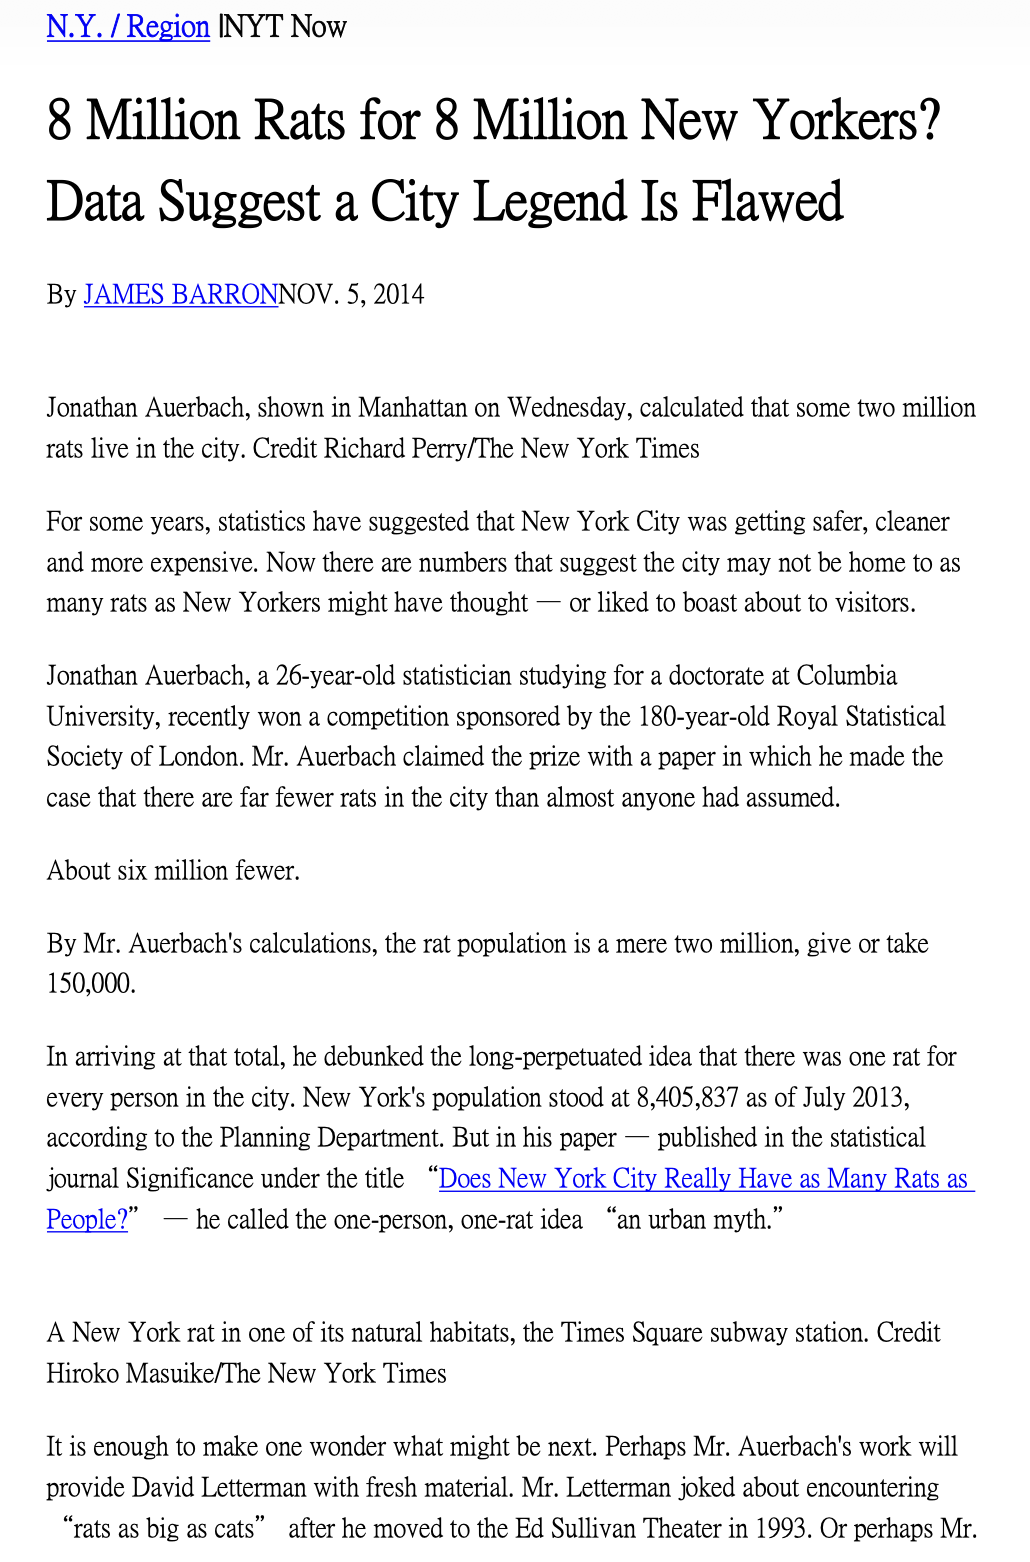
\includegraphics[width=0.88\textwidth,height=1.1\textheight,keepaspectratio]{images/2014_q4_article_1.png}
    \end{center}
}{}
\IfFileExists{images/2014_q4_article_2.png}{%
    \begin{center}
    
\includegraphics[width=0.88\textwidth,height=1.1\textheight,keepaspectratio]{images/2014_q4_article_2.png}
    \end{center}
}{}
\IfFileExists{images/2014_q4_article_3.png}{%
    \begin{center}
    
\includegraphics[width=0.88\textwidth,height=0.8\textheight,keepaspectratio]{images/2014_q4_article_3.png}
    \end{center}
}{}

\bigskip

\textbf{Q5. [15 + 5]} \textbf{\textcolor{red}{Chapter 14}} (A Little More Theory)

\textbf{(i)} Consider the MLE of $\theta$, $\hat\theta$. Using the result that $\hat\theta\overset{p}{\longrightarrow}\theta$, show
\[
\sqrt n(\hat\theta-\theta)\overset{D}{\longrightarrow}N\!\left(0,1/\nu(\theta)\right),
\]
where
\[
\nu(\theta)=E\left[\frac{d\log f(x,\theta)}{d\theta}\right]^2
=E\left[-\frac{d^2\log f(x,\theta)}{d\theta^2}\right].
\]

In your proof you must state all the assumptions, and results you use. [Hint: Use the following Taylor series expansion:
\[
0=\left.\frac{1}{n}\frac{dl(\theta)}{d\theta}\right|_{\hat\theta}
=\frac{1}{n}\frac{dl(\theta)}{d\theta}
+\left.\frac{1}{n}\frac{d^2l(\theta)}{d\theta^2}\right|_{\theta^*}
(\hat\theta-\theta),
\]
where $l(\theta)$ is the log-likelihood function and $\theta^*$ lies between the true value $\theta$ and $\hat\theta$].

\textbf{(ii)} Interpret the result in (i) in terms of efficiency of $\hat\theta$.

\bigskip

\textbf{Q6. [10]} \textbf{\textcolor{red}{Chapter 15}} (``Testing'' the Tests)

Given the p.d.f.
\[
f(y)=\begin{cases}
\dfrac{1}{\theta}, & 0<y\leq\theta,\\[3pt]
0, & \text{otherwise}.
\end{cases}
\]

Our problem is to test the hypothesis $H_0:\theta=2$ against $\theta=4$, having only a single observation ``$y$''. Two tests are suggested:

\textbf{A.} Reject $H_0$, if $y\geq 1$.

\textbf{B.} Reject $H_0$, if $y\geq 1.5$.

Compare these two tests in terms of their type-I and type-II error probabilities.

\bigskip

\textbf{Q7. [10]} (Epilogue: Closing the Course with a ``Bright'' Note)

State one result (with proof) from this course that you found most interesting.

[Hint: Use only the space between the two dotted lines below]


% ============================================================
% 2013 FINAL (append before \end{document})
% ============================================================
\clearpage

\begin{center}
    {\Large\bfseries 2013 Final}
\end{center}

\vspace{1em}

\textbf{Q1. [15]} \textbf{\textcolor{red}{Chapter 9}}

Given a random sample $\{X_1,X_2,\ldots,X_n\}$ from the population $N(\mu,\sigma^2)$, define
\[
\overline X=\frac{\sum_{i=1}^n X_i}{n}, \qquad
S^2=\frac{1}{n}\sum_{i=1}^n(X_i-\overline X)^2,
\]
\[
S^{\prime 2}=\frac{1}{n-1}\sum_{i=1}^n(X_i-\overline X)^2
\quad\text{and}\quad
S_0^2=\frac{1}{n}\sum_{i=1}^n(X_i-\mu)^2.
\]

In the class, we proved that $\overline X$ and $S^2$ are independent, and they are distributed as, respectively,
\[
\overline X\sim N\!\left(\mu,\frac{\sigma^2}{n}\right),
\qquad \frac{nS^2}{\sigma^2}\sim\chi^2_{n-1}.
\]

Utilizing these results derive the distributions (expressions of pdfs are not required) of
\[
\frac{\sqrt n(\overline X-\mu)}{S'},\quad
\frac{\sqrt n(\overline X-\mu)}{S},\quad
\frac{n(S_0^2-S^2)}{\sigma^2},
\]
\[
\left[\frac{\sqrt n(\overline X-\mu)}{\sigma}\right]^2
+\frac{nS^2}{\sigma^2},
\qquad\text{and}\qquad
\frac{n(\overline X-\mu)^2}{S^{\prime 2}}.
\]

\bigskip

\textbf{Q2. [15]}

Multiple choice questions: for this part circle your choice clearly. There are 5 questions each with 3 marks.

\textbf{(i)} Let the random variable $X_n$ be given by
\[
\begin{aligned}
X_n&=1\ \text{with probability }a^n,\quad 0<a<1,\\
&=0\ \text{with probability }1-a^n.
\end{aligned}
\]
Then the sequence $\{X_n\}$ converges in probability to
\begin{enumerate}
\setlength{\itemsep}{0pt}\setlength{\parsep}{0pt}\setlength{\topsep}{2pt}
\item[A.] $-1$
\item[B.] $+1$
\item[C.] $0$
\item[D.] $a$
\item[E.] None of the above
\end{enumerate}

\textbf{(ii)} An estimator $\hat\theta_n$ based on a sample of $n$ is said to be consistent for $\theta$ if
\begin{enumerate}
\setlength{\itemsep}{0pt}\setlength{\parsep}{0pt}\setlength{\topsep}{2pt}
\item[A.] $\displaystyle\lim_{n\to\infty}\Pr(|\hat\theta_n-\theta|>\varepsilon)=1$ for any $\varepsilon>0$
\item[B.] $\displaystyle\lim_{n\to\infty}\operatorname{MSE}(\hat\theta_n)=0$
\item[C.] $\displaystyle\lim_{n\to\infty}E(\hat\theta_n)=0$
\item[D.] $\displaystyle\lim_{n\to\infty}V(\hat\theta_n)=0$
\item[E.] None of the above.
\end{enumerate}

\textbf{(iii)} Using the notations of Q.1, which statement below is \emph{not} correct.
\begin{enumerate}
\setlength{\itemsep}{0pt}\setlength{\parsep}{0pt}\setlength{\topsep}{2pt}
\item[A.] $\displaystyle\operatorname{plim}_{n\to\infty}S'=\sigma$
\item[B.] $\displaystyle E(S^{\prime 2})=\operatorname{plim}_{n\to\infty}S^2=\sigma^2$
\item[C.] $\displaystyle E(S')=\sigma$
\item[D.] $\displaystyle E(S^2)=\frac{n-1}{n}\sigma^2$
\item[E.] $\displaystyle\operatorname{plim}_{n\to\infty}S=\sigma$
\end{enumerate}

\textbf{(iv)} Let $X_n$, $X$, $Y_n$ and $Y$ be random variables. Then which of the following statement is true?
\begin{enumerate}
\setlength{\itemsep}{0pt}\setlength{\parsep}{0pt}\setlength{\topsep}{2pt}
\item[A.] $\{X_n\xrightarrow{p}X,\ Y_n\xrightarrow{D}Y\}$ implies $\{X_n+Y_n\xrightarrow{p}X+Y\}$
\item[B.] $X_n\xrightarrow{D}X$ implies $X_n\xrightarrow{p}X$
\item[C.] $\{X_n\xrightarrow{p}X,\ Y_n\xrightarrow{p}Y\}$ implies $(X_n,Y_n)\xrightarrow{p}(X,Y)$
\item[D.] $\{X_n\xrightarrow{p}X,\ Y_n\xrightarrow{D}Y\}$ implies $(X_n,Y_n)\xrightarrow{p}(X,Y)$
\item[E.] $\{X_n\xrightarrow{D}X,\ Y_n\xrightarrow{p}Y\}$ implies $(X_n,Y_n)\xrightarrow{p}(X,Y)$
\end{enumerate}

\textbf{(v)} Suppose $l(\theta)$ be the loglikelihood function and $\hat\theta$ be an estimator satisfying
\[
\frac{dl(\theta)}{d\theta}=\frac{\hat\theta-\theta}{Var(\hat\theta)}.
\]
Then $\hat\theta$ is
\begin{enumerate}
\setlength{\itemsep}{0pt}\setlength{\parsep}{0pt}\setlength{\topsep}{2pt}
\item[A.] Only consistent and unbiased.
\item[B.] BLUE (Best Linear Unbiased Estimator)
\item[C.] MVUE (Minimum Variance Unbiased Estimator)
\item[D.] MLE (Maximum Likelihood Estimator)
\item[E.] None of the above.
\end{enumerate}

\bigskip

\textbf{Q3. [10 + 10]} \textbf{\textcolor{red}{Chapter 15}}

Let $X\sim N(\mu,\sigma^2)$ where $\sigma^2$ is known. We want to test $H_0:\mu=\mu_0$ against $H_a:\mu_a>\mu_0$. Using the Neyman-Pearson lemma, the most powerful test is (do not derive this):
\[
\text{Reject }H_0\text{ if }\quad
\frac{\sqrt n(\overline X-\mu_0)}{\sigma}>Z_\alpha.
\]

\textbf{(a)} Show that the power of this test is given by $\Phi(\delta-Z_\alpha)$, where $\delta=\sqrt n(\mu_a-\mu_0)/\sigma$ is a measure of distance between the null and alternative hypothesis. Here $\Phi(\cdot)$ denotes the distribution function of $N(0,1)$.

\textbf{(b)} Draw and interpret the power curve for all $\mu_a\neq\mu_0$.

\bigskip

\textbf{Q4. [5 + 10]} \textbf{\textcolor{red}{Chapter 13}}

Let $\{X_1,X_2,\ldots,X_n\}$ be a random sample from $N(\mu,\sigma^2)$. Show that

\textbf{(a)} when $\sigma^2$ is known, the sample mean $\overline X=\sum_{i=1}^nX_i/n$ is a sufficient statistic for $\mu$.

\textbf{(b)} but when $\mu$ is known, the sample variance $S^2=\frac{1}{n}\sum_{i=1}^n(X_i-\overline X)^2$ is not a sufficient statistic for $\sigma^2$. Suggest a sufficient statistic for $\sigma^2$ for this case.

\bigskip

\textbf{Q5. [5 + 10]} \textbf{\textcolor{red}{Chapter 15}}

A plot of your midterm expected grade ($X$) supplied by you, and observed grade ($Y$) is given in the next page. Here the grades are $C$, $B-$, $B$, $B+$, $A-$, $A$, $A+$ corresponding to levels 1, 2, 3, 4, 5, 6 and 7, respectively.

% Plot of observed versus expected midterm grades (original PDF page 11).
% Add your image to images/2013_q5_grades.png to include it automatically.
\IfFileExists{images/2013_q5.png}{%
\begin{center}
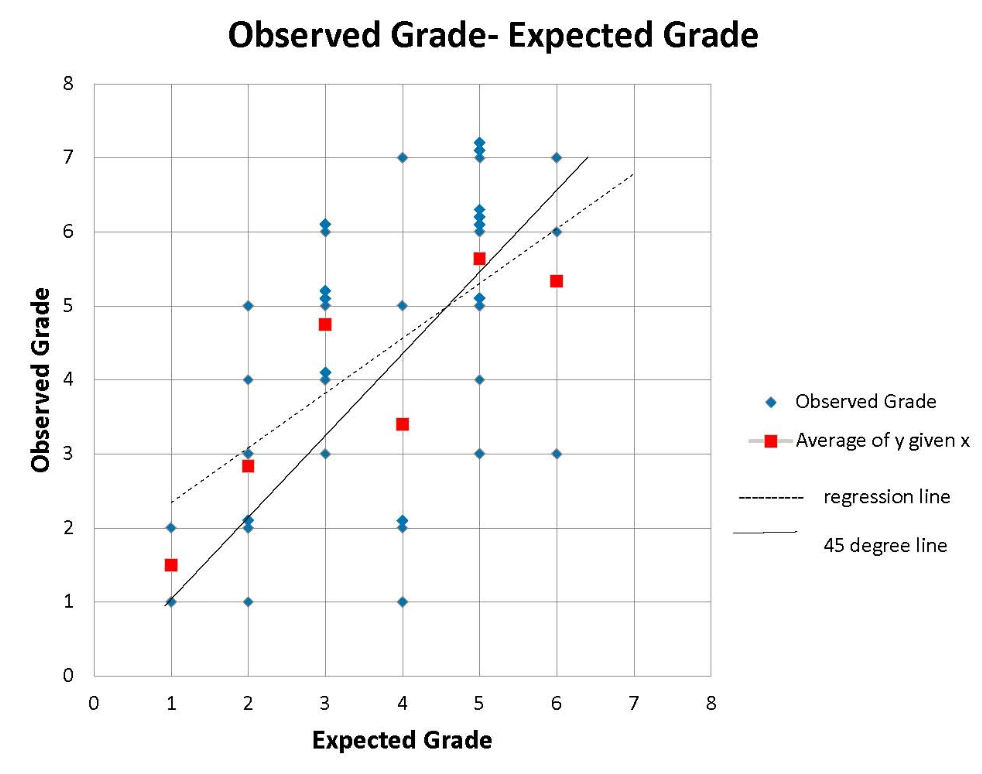
\includegraphics[width=0.80\textwidth,height=0.50\textheight,keepaspectratio]{images/2013_q5.png}
\end{center}
}{}

\textbf{(a)} From the data (sample size, $n=35$) we calculated [again, $X$: expected; $Y$: observed]:
\[
\hat\mu_x=\frac1n\sum_{i=1}^n X_i=3.74,\qquad \hat\mu_y=4.37
\]
\[
\hat\sigma_x^2=\frac1n\sum_{i=1}^n(X_i-\hat\mu_x)^2=2.01,\qquad \hat\sigma_y^2=3.60.
\]
Interpret the differences in sample means and variances of $X$ and $Y$.

\textbf{(b)} When we run the regression $E(Y\mid X)=\alpha+\beta X$, we obtain the following result:
\[
\begin{array}{r@{}c@{}l}
\hat y\;=\;&1.60&{}+\;0.74\,X,\\[-2pt]
& (0.77)&\hspace{0.55em}(0.19)
\end{array}
\]
where the standard errors are given in parentheses. Test the null hypothesis, $H_0:\beta=1.0$ against $H_a:\beta<1.0$. You can use $t_{0.10(33)}=1.30$. Also test $H_0:\alpha=0$ against $H_a:\alpha>0$. Interpret your test results.

\bigskip

\textbf{Q6. [5 + 15]} \textbf{\textcolor{red}{Chapter 15}}

Suppose we want to test $H_0:\theta=\theta_0$ against $H_1:\theta\neq\theta_0$.

\textbf{(i)} Define and simplify the likelihood ratio (LR) (denoting it by $\lambda$) for testing $H_0$ vs. $H_1$.

\textbf{(ii)} Show (step-by-step) that under $H_0$:
\[
-2\log_e\lambda\xrightarrow{D}\chi_1^2.
\]
[Hint: Use the following Taylor series expansion
\[
\ell(\theta_0)=\ell(\hat\theta)+(\theta_0-\hat\theta)
\left.\frac{\partial\ell(\theta)}{\partial\theta}\right|_{\hat\theta}
+\frac12(\theta_0-\hat\theta)^2
\left.\frac{\partial^2\ell(\theta)}{\partial\theta^2}\right|_{\theta^*},
\]
where $\ell(\theta)$ is the loglikelihood function, $\hat\theta$ is the MLE, and $\theta^*$ lies between $\theta_0$ and $\hat\theta$.] In your proof, you must state all the results that you use.



% ============================================================
% 2012 FINAL (append before \end{document})
% ============================================================
\clearpage

\begin{center}
    {\Large\bfseries 2012 Final}
\end{center}

\vspace{1em}

\textbf{Q1. [15]} \textbf{\textcolor{red}{Chapter 9}}

Given a random sample $\{X_1,X_2,\ldots,X_n\}$ from the population $N(\mu,\sigma^2)$, define
\[
\overline X=\frac{\sum_{i=1}^{n}X_i}{n},\qquad
S^2=\frac{1}{n}\sum_{i=1}^{n}(X_i-\overline X)^2,
\]
and
\[
S^{\prime 2}=\frac{1}{n-1}\sum_{i=1}^{n}(X_i-\overline X)^2.
\]

In the class, we proved that $\overline X$ and $S^2$ are independent, and they are distributed as, respectively,
\[
\overline X\sim N\!\left(\mu,\frac{\sigma^2}{n}\right),\qquad
\frac{nS^2}{\sigma^2}\sim\chi_{n-1}^2.
\]

Utilizing these results find (only short derivations are required) the distributions of the following random variables: For example, since $\overline X\sim N\!\left(\mu,\frac{\sigma^2}{n}\right)$, $\dfrac{\sqrt{n}(\overline X-\mu)}{\sigma}\sim N(0,1)$.

\begin{enumerate}
\item[(i)] $\displaystyle \frac{\sqrt{n}\,\overline X}{\sigma}$
\item[(ii)] $\displaystyle \frac{(n-1)S^{\prime 2}}{\sigma^2}$
\item[(iii)] $\displaystyle \frac{\sqrt{n-1}(\overline X-\mu)}{S}$
\item[(iv)] $\displaystyle \frac{\sqrt n(\overline X-\mu)}{S'}$
\item[(v)] $\displaystyle \sqrt{n}(\overline X-\mu)$
\end{enumerate}

\bigskip

\textbf{Q2. [5 + 5 + 5 + 5 + 5 + 10]} \textbf{\textcolor{red}{Chapters 12}}

\begin{enumerate}
\item[(a)] Define the concept of ``convergence in probability.''

\item[(b)] What is the connection between ``convergence in probability'' and ``consistency of an estimator $\hat\theta$ for a parameter $\theta$''?

\item[(c)] Utilizing the inequality that for any non-negative continuous function $g(X)$ of a random variable $X$, assuming $E[g(X)]$ exists;
\[
\Pr[g(X)\geq\varepsilon^2]\leq\frac{E[g(X)]}{\varepsilon^2},
\]
Prove that
\[
\Pr[|\hat\theta-\theta|<\varepsilon]\geq 1-\frac{E(\hat\theta-\theta)^2}{\varepsilon^2},
\]
for any $\varepsilon>0$.

\item[(d)] From (c), derive the sufficient condition(s) for an estimator $\hat\theta$ to be consistent for a parameter $\theta$.

\item[(e)] Let $X_i\sim\mathrm{IID}(\mu,\sigma^2)$, $i=1,2,\ldots,n$. Using your results in (d), check the consistency of $\overline X=\sum_{i=1}^{n}X_i/n$ for $\mu$.

\item[(f)] Same as in (e), but now relax the independence of $X_i$'s with $Corr(X_i,X_j)=\rho$, $i\neq j$, $i,j=1,2,\ldots,n$. Now check the consistency of $\overline X$.
\end{enumerate}

\bigskip

\textbf{Q3. [15]} \textbf{\textcolor{red}{Chapter 13}}

Prove the Rao-Blackwell theorem as stated below:

Let $U$ be an unbiased estimator and $T$ be a sufficient statistic for $\theta$. Define $V(T)=E(U\mid T)$. Then

(i) $E[V(T)]=\theta$ and (ii) $Var[V(T)]\leq Var(U)$.

Notations are as used in the class. But you should explain the notations and introduce new ones as needed, and state the required assumptions.

\bigskip

\textbf{Q4. [20]} \textbf{\textcolor{red}{Chapter 15}}

Suppose we want to test $H_0:\theta=\theta_0$ against $H_1:\theta\neq\theta_0$. Define $\lambda$ as the likelihood ratio (LR): $\lambda=\dfrac{L(\theta_0)}{L(\hat\theta)}$, where $\hat\theta$ is the maximum likelihood estimator (MLE) of $\theta$.

Show that under $H_0$:
\[
-2\log_e\lambda\xrightarrow{D}\chi_1^2.
\]

\bigskip

\textbf{Q5. [10]}

Write a short note on the Life \& Work of any one of the following (in \emph{maximum} 10 sentences):

\begin{enumerate}
\item[(i)] Karl Pearson
\item[(ii)] R.A. Fisher
\item[(iii)] Jerzy Neyman
\item[(iv)] Egon Pearson
\item[(v)] C.R. Rao
\item[(vi)] David Blackwell
\end{enumerate}

\bigskip

\textbf{Q6. [5]}

We all watched the documentary on the life and work of P.C. Mahalanobis. There we learned about the myriad of application of Statistics to fields like, Biology, Anthropology, Psychology, Industry, Flood Control, Forensic Science, Space Research, Health Science, Wealth Forecasting and Economic Planning. Elaborate on the importance of Statistics to one of these fields (in \emph{maximum} 5 sentences).



% ============================================================
% 2009 FINAL (append before \end{document})
% ============================================================
\clearpage

\begin{center}
    {\Large\bfseries 2009 Final}
\end{center}

\vspace{1em}

\textbf{Q1. [10 + 5 + 5]} \textbf{\textcolor{red}{Chapter 11}}

The ideal size of the first year Econ Ph.D. class at UIUC is thought to be 20. From the earlier years' data it is known that on the average 50\% students accepts the admission offer. Suppose for the 2010-11 academic year, 40 students are offered admission. Then what is the probability that more than 25 students will actually join? [Hint: You can use, $\Phi(1.58)\approx 0.94$.] State all the assumptions and the \emph{results}, you are using.

\bigskip

\textbf{Q2. [10 + 5 + 5 + 10 + 5]} \textbf{\textcolor{red}{Chapter 11}}

Let $X\sim N(\mu,\sigma^2)$.

\begin{enumerate}
\item[(a)] Derive the $2\times 2$ information matrix $I(\theta)$, where
\[
\theta=\begin{pmatrix}\mu\\\sigma^2\end{pmatrix},
\]
using a random sample $\{X_1,X_2,\ldots,X_n\}$.

\item[(b)] Interpret the components of $I(\theta)$.

\item[(c)] Discuss the role of $I(\theta)$ for the Cram\'er-Rao lower bound.

\item[(d)] Now \emph{relax} the normality assumption, and only assume that $E(X)=\mu$, $Var(X)=\sigma^2$, $E(X-\mu)^3=\mu_3$ and $E(X-\mu)^4=\mu_4$. Derive the information matrix under this set up.

\item[(e)] Under what conditions, the information matrices derived in (a) and (d) are the same?
\end{enumerate}

\bigskip

\textbf{Q3. [5 + 15]} \textbf{\textcolor{red}{Chapter 15}}

Suppose we want to test $H_0:\theta=\theta_0$ against $H_1:\theta\neq\theta_0$. Define $\lambda$ as the appropriate likelihood ratio (LR). Show that under $H_0$:
\[
-2\log_e\lambda\xrightarrow{D}\chi_1^2.
\]
[Hint: Use the following Taylor series expansion
\[
\ell(\theta)=\ell(\hat\theta)
+(\theta-\hat\theta)\left.\frac{\partial\ell(\theta)}{\partial\theta}\right|_{\hat\theta}
+\frac{1}{2}(\theta-\hat\theta)^2
\left.\frac{\partial^2\ell(\theta)}{\partial\theta^2}\right|_{\theta^*},
\]
where $\ell(\theta)$ is the loglikelihood function, $\hat\theta$ is the MLE, and $\theta^*$ lies between the true value $\theta$ and $\hat\theta$.] In your proof, you must state \emph{all the results} that you use.

\clearpage

\textbf{Q4. [5 + 15 + 5]} \textbf{\textcolor{red}{Chapter 15}}

A plot of your midterm expected grade ($X$) supplied by you, and observed grade ($Y$) is given in the next page. Here the grades are $C,B-,B,B+,A-,A,A+$ corresponding to levels 1, 2, 3, 4, 5, 6 and 7, respectively. In the plot, ``o'' denotes the data point for each $(X,Y)$ pair, and multiple observations on some locations are lumped together.

% Original scatter plot is on page 10 of Econ506_Final_2009_Answers.pdf.
% Save the plot as images/2009_q4_grades.png to include it automatically.
\IfFileExists{images/2009_q4.png}{%
\begin{center}
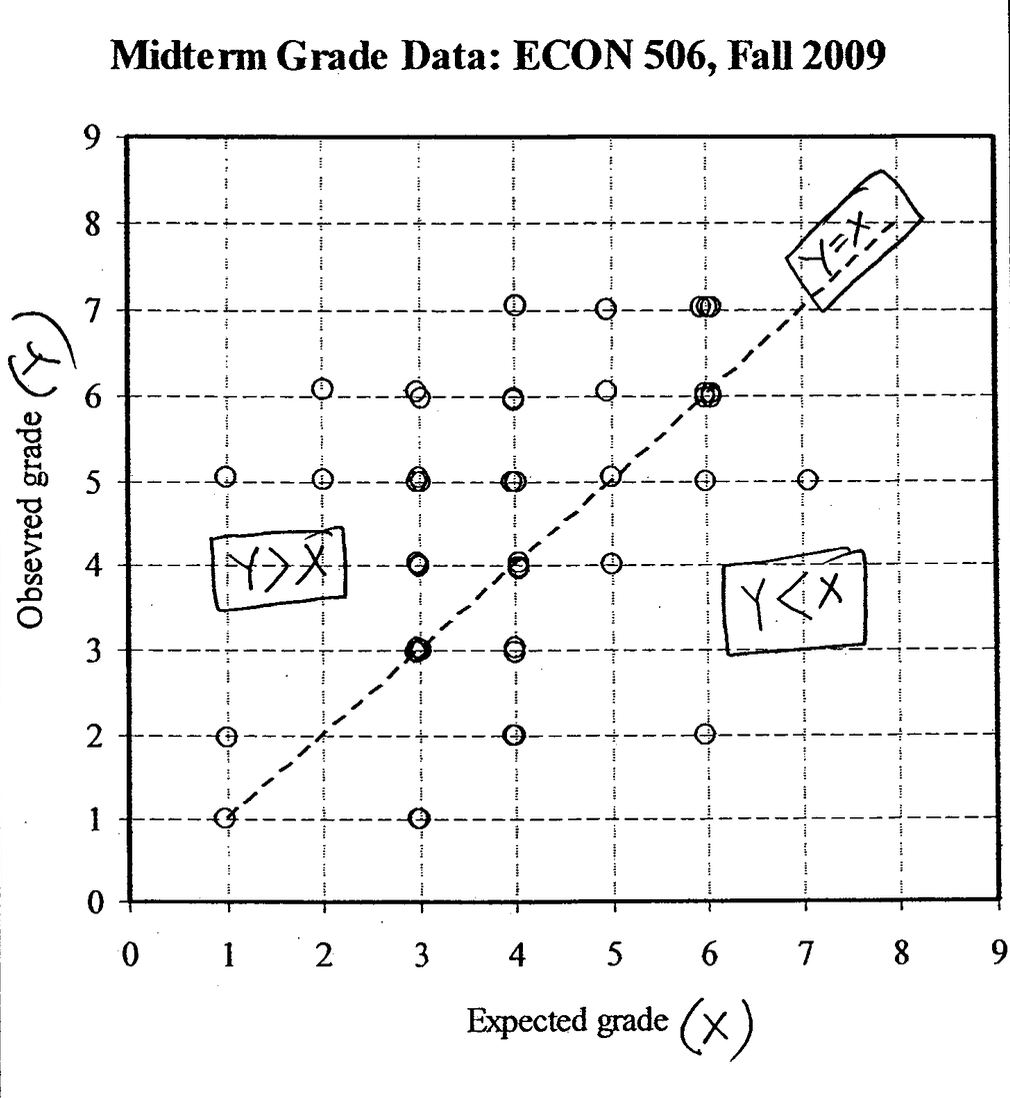
\includegraphics[width=0.80\textwidth,height=0.50\textheight,keepaspectratio]{images/2009_q4.png}
\end{center}
}{}

\begin{enumerate}
\item[(a)] From the scatter plot, how would you characterize students' expectations (optimistic, pessimistic or unbiased) in relation to their actual performance? Explain your answer.

\item[(b)] From the data (sample size, $n=48$) we calculated [again, $X$: expected; $Y$: observed]:
\[
\begin{aligned}
\hat\mu_x &= \frac{1}{n}\sum_{i=1}^n X_i =3.93,
&\qquad \hat\mu_y&=4.39,\\[3pt]
\hat\sigma_x^2&=\frac{1}{n}\sum_{i=1}^n(X_i-\hat\mu_x)^2=2.10,
&\qquad \hat\sigma_y^2&=3.01,\\[3pt]
\hat\sigma_{xy}&=\frac{1}{n}\sum_{i=1}^n(X_i-\hat\mu_x)(Y_i-\hat\mu_y)=1.087,\\[3pt]
\hat\rho_{xy}&=\hat\sigma_{xy}/(\hat\sigma_x\hat\sigma_y)=0.441.
\end{aligned}
\]
Test the hypothesis $H_0:\mu_y=\mu_x$ against $H_a:\mu_y>\mu_x$. State all your assumptions, and discuss the result of the test. [You can use the critical values $t_{0.10;47}=1.300$, $t_{0.05;47}=1.678$ and $t_{0.01;47}=2.408$.]

\item[(c)] How would you interpret $\hat\sigma_x^2<\hat\sigma_y^2$?
\end{enumerate}


% ============================================================
% 2008 FINAL (append before \end{document})
% ============================================================
\clearpage

\begin{center}
    {\Large\bfseries 2008 Final}
\end{center}

\vspace{1em}

\textbf{Q1. [8 + 12 + 10]} \textbf{\textcolor{red}{Chapters 9}}

Given a random sample $\{X_1,X_2,\ldots,X_n\}$ from the population $N(\mu,\sigma^2)$, define
\[
\overline X=\frac{\sum_{i=1}^{n}X_i}{n},\qquad
S^2=\frac{1}{n}\sum_{i=1}^{n}(X_i-\overline X)^2,
\]
\[
S'^2=\frac{1}{n-1}\sum_{i=1}^{n}(X_i-\overline X)^2
\quad\text{and}\quad
S_0^2=\frac{1}{n}\sum_{i=1}^{n}(X_i-\mu)^2.
\]

In the class, we proved that $\overline X$ and $S^2$ are independent, and they are distributed as, respectively,
\[
\overline X\sim N\!\left(\mu,\frac{\sigma^2}{n}\right)
\quad\text{and}\quad
\frac{nS^2}{\sigma^2}\sim\chi^2_{n-1}.
\]

\begin{enumerate}
\item[(i)] Using the above results, find the distribution of $\dfrac{nS_0^2}{\sigma^2}$. Then compare the variances of $S^2$ and $S_0^2$ and explain your result.

\item[(ii)] Find the distributions of the following statistics (derivations are not required):
\[
\frac{\sqrt n\,\overline X}{\sigma},\quad
\frac{\sqrt n\,(\overline X-\mu)}{S},\quad
\frac{\sqrt{n-1}(\overline X-\mu)}{S'},\quad\text{and}\quad
\frac{\sqrt n\,(\overline X-\mu)}{S'}.
\]

\item[(iii)] Suppose we want to test $H_0:\mu=0$ against $H_a:\mu\neq 0$. The likelihood ratio (LR) test for this problem, with size $\alpha$, is to reject $H_0$ if
\[
\left|\frac{\sqrt n\,\overline X}{S'}\right|>t_{\alpha/2,n-1}.
\]
Discuss the power (function) of this test.
\end{enumerate}

\bigskip

\textbf{Q2. [5 + 15 + 5 + 5 + 5]} \textbf{\textcolor{red}{Chapter 15}}

Data on the grades [(Observed, Expected): 8 is highest, 1 lowest] of your midterm exam are given below ($n=35$):

\begin{quote}\small
(8,8), (6,6), (8,8), (3,2), (9,6), (8,6), (1,2), (4,1),
(8,8), (5,7), (8,8), (7,7), (8,7), (8,7), (6,2), (7,7),
(1,4), (8,6), (8,7), (4,1), (8,5), (2,2), (8,5), (8,8),
(8,7), (8,6), (8,7), (4,5), (8,5), (7,6), (8,7), (7,7),
(5,6), (5,4), (6,4).
\end{quote}

The sample means and variances (using the formula $\frac1n\sum_{i=1}^n(X_i-\overline X)^2$) are:

\begin{center}
\begin{tabular}{|l|c|c|}
\hline
 & Observed & Expected \\
\hline
Mean & 6.43 & 5.54 \\
Variance & 4.70 & 4.36 \\
\hline
\end{tabular}
\end{center}

\begin{enumerate}
\item[(i)] Comment on the above ``lower'' sample values for the ``Expected'' grades.

\item[(ii)] Using the above data, test whether the expected and observed grades have the same mean. State your assumptions clearly.

\item[(iii)] Comment on the validity of carrying out formal statistical test(s) on data collected in the class (the way we did).

\item[(iv)] To gain further insight on the distribution of grades, we plot the kernel densities below:

% Original plot is on page 5 of Econ506_Final_2008_Answers.pdf.
% Save it as images/2008_q2_kernel_densities.png to include it automatically.
\IfFileExists{images/2008_q2.png}{%
\begin{center}
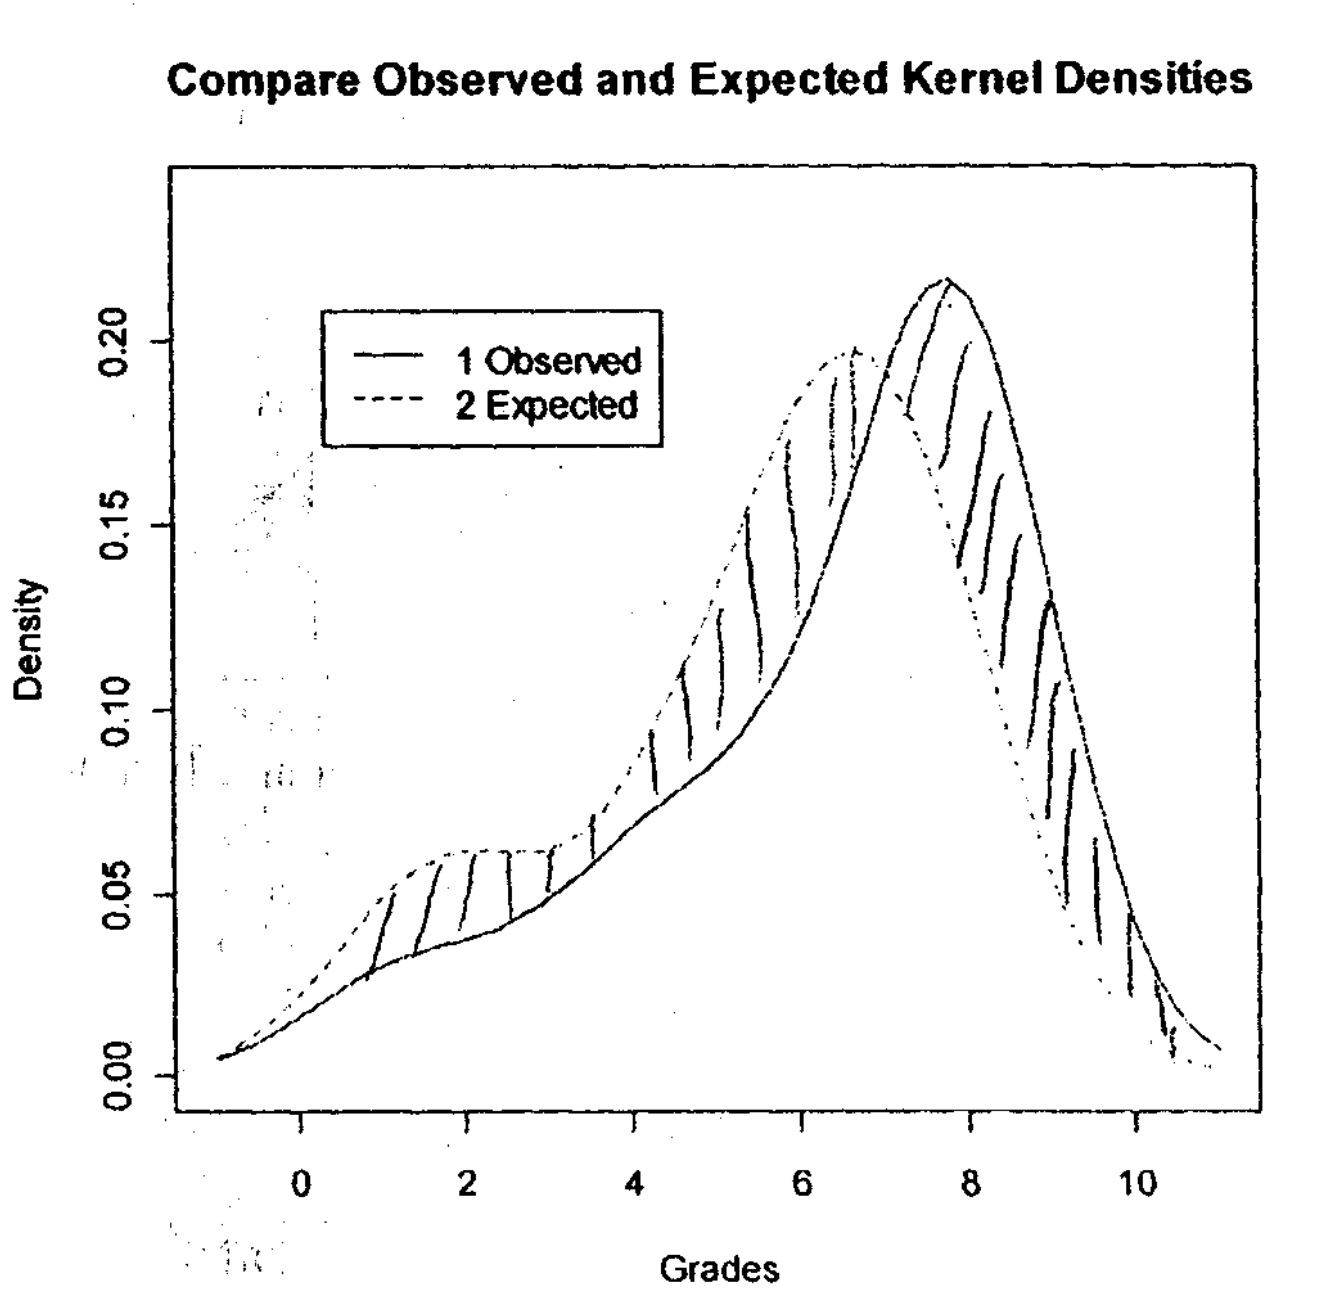
\includegraphics[width=0.80\textwidth,height=0.40\textheight,keepaspectratio]{images/2008_q2.png}
\end{center}
}{}

What can you say about the skewness and kurtosis of these two densities?

\item[(v)] Indicate how would you go about testing the equality of these two distributions. (No formal derivation is required).
\end{enumerate}

\bigskip

\textbf{Q3. [15 + 10]} \textbf{\textcolor{red}{Chapter 10}}

\begin{enumerate}
\item[(a)] Let $X_1,X_2,\ldots,X_n$ be a random sample of size $n$ from an univariate population with distribution function $F(x)$ and central moments
\[
\mu_k=\int (x-\mu)^k\,dF(x),\qquad k=2,3,\ldots
\]
where $E(x)=\mu$. Let $\overline X$ and $S^2=\frac1n\sum_{i=1}^n(X_i-\overline X)^2$ denote the sample mean and variance, respectively. Then show that
\[
\sqrt n\,(S^2-\mu_2)\xrightarrow{D}N(0,\mu_4-\mu_2^2).
\]

\item[(b)] Now assume that $\{X_i\}$'s are $IIDN(\mu,\sigma^2)$, $i=1,2,\ldots,n$. Then find the finite sample and asymptotic distributions of $\sqrt n\,(S^2-\mu_2)$.
\end{enumerate}

\bigskip

\textbf{Q4. [5 + 10]} \textbf{\textcolor{red}{Chapter 11}}

An ``Outline'' of a proof a ``Result'' is given below. Write down the ``Result''. Discuss \underline{one} situation when this ``Result'' will not hold.

\textbf{Answer:} We have
\[
L(\theta)=\prod_{i=1}^n f(x_i,\theta),
\]
\[
\text{i.e.}\quad \log L(\theta)=\sum_{i=1}^n\log f(x_i,\theta),
\]
\[
\text{i.e.}\quad \frac{d\log L(\theta)}{d\theta}
=\sum_{i=1}^n\frac{d\log f(x_i,\theta)}{d\theta}.
\]

Now square both sides and take expectations, assuming $f(x;\theta)$ as the true density. From the right hand side, we have
\[
E\!\left[\sum_{i=1}^n\frac{d\log f(x_i,\theta)}{d\theta}\right]^2
=\sum_{i=1}^n E\!\left[\frac{d\log f(x_i,\theta)}{d\theta}\right]^2
=nE\!\left[\frac{d\log f(x_i,\theta)}{d\theta}\right]^2.
\qquad (\text{Q.E.D.})
\]

% ============================================================
% 2007 FINAL (append before \end{document})
% ============================================================
\clearpage

\begin{center}
    {\Large\bfseries 2007 Final}
\end{center}

\vspace{1em}

\textbf{Q1. [20 + 10]} \textbf{\textcolor{red}{Chapter 9}}

Let $X_1,X_2,\ldots,X_n$ be a random sample from a population with finite third central moment $\mu_3$. Define the sample mean and variance, respectively, as
\[
\overline X=\frac{\sum_{i=1}^n X_i}{n}
\quad\text{and}\quad
S^2=\frac{1}{n}\sum_{i=1}^n(X_i-\overline X)^2.
\]

\begin{enumerate}
\item[(a)] Show that
\[
\operatorname{Cov}(\overline X,S^2)=\left(\frac{n-1}{n^2}\right)\mu_3.
\]

\item[(b)] ``Therefore, under normality, $\operatorname{Cov}(\overline X,S^2)=0$. If we take the random variable $X$ as return of an investment, then we can interpret $\overline X$ and $S^2$, respectively, as average ``return'' and ``risk''. Therefore, we can conclude that there is no relationship between risk and return.''

Discuss the above argument whichever way you see fit.
\end{enumerate}

\bigskip

\textbf{Q2. [10]} \textbf{\textcolor{red}{Chapter 10}}

Let $Z_i\sim\operatorname{IID}N(0,1)$, $i=1,2,\ldots,n$. Define $Y_i=Z_i^2$ and $\overline S_n=\frac1n\sum_{i=1}^n Y_i$.

Find the asymptotic distribution of
\[
\frac{\sqrt n\,(\overline S_n-1)}{\sqrt 2}.
\]

\bigskip

\textbf{Q3. [20 + 5]} \textbf{\textcolor{red}{Chapter 11}}

\begin{enumerate}
\item[(a)] Suppose the density function $f(y;\theta)$ satisfies the regularity conditions, and $T$ be an unbiased estimator of $\psi(\theta)$ which is differentiable in $\theta$. Then show that
\[
\operatorname{Var}(T)\geq [I(\theta)]^{-1}
\left(\frac{d\psi(\theta)}{d\theta}\right)^2, \tag{1}
\]
where $I(\theta)$ is the information in the sample.

\item[(b)] From (1) derive the Cram\'er--Rao inequality.
\end{enumerate}

\bigskip

\textbf{Q4. [5 + 5]} \textbf{\textcolor{red}{Chapter 15}}

In Neyman-Pearson test principle, we fix the type-I error probability ($\alpha$) at a low level and then minimize the type-II error probability ($\beta$). How would you justify that? Under what circumstances minimization of $\alpha$ after fixing $\beta$ at a low level would be justified?

\bigskip

% The original exam labels this question "4" again; numbering is preserved.
\newpage
\textbf{Q4. [15 + 10]} \textbf{\textcolor{red}{Chapter 15}}

\begin{enumerate}
\item[(a)] Let $X_1,X_2,\ldots,X_n$ denote a random sample of size $n$ from the Bernoulli distribution,
\[
f(x,p)=p^x(1-p)^{1-x},\qquad x=0,1.
\]
Find the best critical region for testing $H_0:p=p_0$ against $H_a:p>p_0$. Hint: Use Neyman-Pearson Lemma.

\item[(b)] Let $n=5$, $p_0=0.6$ and $\alpha=\Pr(\text{Type-I error})=0.05$. Find the \emph{exact} critical value for the test derived in Part (a).

Hint: When $Y\sim\operatorname{Binomial}(5,0.6)$, it has the following probability distribution:
\begin{center}
\begin{tabular}{c|cccccc}
$y$ & 0 & 1 & 2 & 3 & 4 & 5 \\ \hline
$\Pr(Y=y)$ & 0.01 & 0.08 & 0.23 & 0.34 & 0.26 & 0.08
\end{tabular}
\end{center}
\end{enumerate}


% ============================================================
% 2006 FINAL (append before \end{document})
% Original: Economics 506, Anil K. Bera, December 11, 2006
% Only the questions are transcribed; handwritten answers are excluded.
% ============================================================
\clearpage

\begin{center}
    {\Large\bfseries 2006 Final}
\end{center}

\vspace{1em}

\begin{center}
\textbf{Part A}
\end{center}

Multiple choice questions: for this part circle your choice clearly.

\textbf{Q1. [5]}

Suppose we have only one observation $y$ from the distribution $Y\sim N(\theta,1)$. We wish to test the hypothesis
\[
H_0:\theta=0\quad\text{against}\quad H_a:\theta>0,
\]
using a test procedure with rejection region $y\geq\frac12$. Then the level of significance of the test is approximately
\begin{enumerate}
\item[(a)] 0.05
\item[(b)] 0.50
\item[(c)] 0.69
\item[(d)] 0.31
\item[(e)] 0.51
\end{enumerate}

\bigskip

\textbf{Q2. [5]}

Let $X_1,X_2,\ldots,X_n$ be a random sample from Poisson distribution with parameter $\theta$. Then an unbiased estimator of $\theta^2$ is given by
\begin{enumerate}
\item[(a)] $\displaystyle\frac{1}{n-1}\sum_{i=1}^{n}(X_i-\overline X)^2$
\item[(b)] $\displaystyle\overline X^2$
\item[(c)] $\displaystyle\frac{1}{n}\sum_{i=1}^{n}X_i^2-\overline X$
\item[(d)] $\displaystyle\frac{1}{n}\sum_{i=1}^{n}X_i^2+\overline X$
\item[(e)] None of the above
\end{enumerate}

\bigskip

\textbf{Q3. [5]}

Suppose $X_1,X_2,\ldots,X_n$ follow an IID Weibull distribution
\[
f(x)=\frac{1}{\alpha}\beta x^{\beta-1}\exp[-x^{\beta}/\alpha],
\qquad 0<x<\infty
\]
with known $\beta(>0)$. Then the sufficient statistic for $\alpha$ is
\begin{enumerate}
\item[(a)] $\displaystyle\sum_{i=1}^{n}(x_i^{\beta})$
\item[(b)] $\displaystyle\prod_{i=1}^{n}(x_i^{\beta})$
\item[(c)] $\displaystyle\sum_{i=1}^{n}x_i$
\item[(d)] Sufficient statistic for $\alpha$ does not exist
\item[(e)] None of the above
\end{enumerate}

\bigskip

\begin{center}
\textbf{Part B}
\end{center}

Write down your answers in the space provided.

\textbf{Q1. [15 + 10]} \textbf{\textcolor{red}{Chapter 10}}

\begin{enumerate}
\item[(a)] Let $X_1,X_2,\ldots,X_n$ be a random sample of size $n$ from an univariate population with distribution function $F(x)$ and central moments
\[
\mu_k=\int (x-\mu)^k\,dF(x),\qquad k=2,3,\ldots
\]
where $E(X)=\mu$. Let $\overline X$ and $S^2=\frac1n\sum_{i=1}^{n}(X_i-\overline X)^2$ denote the sample mean and variance, respectively. Then show that
\[
\sqrt n\,(S^2-\mu_2)\xrightarrow{D}N(0,\mu_4-\mu_2^2).
\]

\item[(b)] Now assume that $\{X_i\}$'s are $IIDN(\mu,\sigma^2)$, $i=1,2,\ldots,n$. Then find the finite sample and asymptotic distributions of $\sqrt n\,(S^2-\mu_2)$.
\end{enumerate}

\bigskip

\textbf{Q2. [10 + 5 + 5]} \textbf{\textcolor{red}{Chapter 14}}

Suppose $X_1,X_2,\ldots,X_n$ is a random sample from the following distribution
\[
f(x)=\theta e^{-x\theta},\qquad 0<x<\infty.
\]
\begin{enumerate}
\item[(a)] Derive the maximum likelihood (ML) and method of moment (MM) estimators for $\theta$. Compare these two estimators.
\item[(b)] Prove that the MLE is a function of the minimal sufficient statistic.
\item[(c)] Check whether the MLE is MVUE of $\theta$.
\end{enumerate}

\bigskip

\textbf{Q3.} \textbf{\textcolor{red}{Chapter 15}}

Let $X\sim N(\mu,\sigma^2)$ where $\sigma^2$ is known. We want to test $H_0:\mu=\mu_0$ against $H_a:\mu<\mu_0$. Using the Neyman-Pearson lemma, the most powerful test is
\[
\text{Reject }H_0\text{ if }\frac{\sqrt n(\overline X-\mu_0)}{\sigma}<-Z_\alpha,
\quad\text{and accept }H_0\text{ otherwise.}
\]
\begin{enumerate}
\item[(a)] \textbf{[10]} Derive the power function of this test.
\item[(b)] \textbf{[5 + 5]} Show that the test is consistent and it possesses the monotonicity property.
\item[(c)] \textbf{[3 + 2]} Investigate the effects of $\sigma^2$ and the significance level $\alpha$ on the power function.
\end{enumerate}

\bigskip

\textbf{Q4. [15 + 10]} \textbf{\textcolor{red}{Chapter 15}}

\begin{enumerate}
\item[(a)] Let $X_1,X_2,\ldots,X_n$ denote a random sample of size $n$ from the Bernoulli distribution,
\[
f(x,p)=p^x(1-p)^{1-x},\qquad x=0,1.
\]
Find the best critical region for testing $H_0:p=p_0$ against $H_a:p>p_0$. Hint: Use Neyman-Pearson Lemma.

\item[(b)] Let $n=5$, $p_0=0.6$ and $\alpha=\Pr(\text{Type-I error})=0.05$. Find the \emph{exact} critical value for the test derived in a Part (a).

Hint: When $Y\sim\operatorname{Binomial}(5,0.6)$, it has the following probability distribution:
\begin{center}
\begin{tabular}{c|cccccc}
$y$ & 0 & 1 & 2 & 3 & 4 & 5 \\ \hline
$\Pr(Y=y)$ & 0.01 & 0.08 & 0.23 & 0.34 & 0.26 & 0.08
\end{tabular}
\end{center}
\end{enumerate}



% ============================================================
% 2005 FINAL (append before \end{document})
% Original: Economics 506, Anil K. Bera, December 8, 2005
% Source calls it "SECOND EXAMINATION"; this archival section uses "Final".
% Only question material is transcribed. Q4 includes a printed answer to grade.
% Handwritten solutions, markings, and cover illustration are omitted.
% ============================================================
\clearpage

\begin{center}
    {\Large\bfseries 2005 Final}
\end{center}

\vspace{1em}

\begin{center}
\textbf{Part A}
\end{center}

Multiple choice questions: for this part circle your choice clearly.

\textbf{Q1. [5]}

An estimator $\hat\theta_n$ based on a sample of size $n$ is consistent for $\theta$, if
\begin{enumerate}
\item[(a)] $\displaystyle\lim_{n\to\infty}\Pr\{|\hat\theta_n-\theta|\leq\varepsilon\}=0$ for any $\varepsilon>0$
\item[(b)] $\displaystyle\lim_{n\to\infty}\Pr\{|\hat\theta_n-\theta|>\varepsilon\}=0$ for any $\varepsilon>0$
\item[(c)] $E(\hat\theta_n)=\theta$ and $\displaystyle\lim_{n\to\infty}\operatorname{Var}(\hat\theta_n)=0$
\item[(d)] None of the above
\end{enumerate}

\bigskip

\textbf{Q2. [5]}

With a random sample $\{X_1,X_2,\ldots,X_n\}$ from the population $N(\mu,\sigma^2)$ to test $H_0:\mu=\mu_0$, one uses the test statistic
\[
R=\frac{\sum_{i=1}^{n}(X_i-\overline X)^2}{\sum_{i=1}^{n}(X_i-\mu_0)^2}.
\]
Then $\dfrac{nR}{n-1}$ is distributed as
\begin{enumerate}
\item[(a)] $F(n-1,n)$
\item[(b)] $\chi^2_{n-1}/\sigma^2$
\item[(c)] Ratio of two $\chi^2_n$
\item[(d)] None of the above
\end{enumerate}

\bigskip

\begin{center}
\textbf{Part B}
\end{center}

Write down your answers in the space provided.

\textbf{Q1. [5 + 10 + 10]} \textbf{\textcolor{red}{Chapter 9}}

Given a random sample $\{X_1,X_2,\ldots,X_n\}$ for the population $N(0,\sigma^2)$, define
\[
\overline X=\sum_{i=1}^{n}X_i/n
\qquad\text{and}\qquad
S^2=\sum_{i=1}^{n}(X_i-\overline X)^2/n.
\]
\begin{enumerate}
\item[(a)] Derive the p.d.f. of $\overline X$.
\item[(b)] Express $\overline X$ and $S^2$, respectively, as linear and quadratic forms of the vector
\[
X=(X_1,X_2,\ldots,X_n)'.
\]
\item[(c)] Using the result that when $Z\sim N(0,I_n)$, $Z'AZ\sim\chi^2_r$, where $r$ is the rank of the matrix $A$, find the distribution of $S^2$.
\end{enumerate}

\bigskip

\textbf{Q2. [15 + 5 + 5]} \textbf{\textcolor{red}{Chapter 11}}

Let $X\sim N(\mu,\sigma^2)$. Derive the $2\times2$ information matrix $\mathcal I(\theta)$, where $\theta=\begin{pmatrix}\mu\\\sigma^2\end{pmatrix}$, using a random sample $\{X_1,X_2,\ldots,X_n\}$.

Interpret the components of $\mathcal I(\theta)$.

Discuss the role of $\mathcal I(\theta)$ for the Cram\'er--Rao lower bound.

\bigskip

\textbf{Q3. [10 + 20 + 5]} \textbf{\textcolor{red}{Chapter 14}}

Let $X\sim N(\mu,\sigma^2)$. Derive the $2\times2$ information matrix $\mathcal I(\theta)$, where $\theta=\begin{pmatrix}\mu\\\sigma^2\end{pmatrix}$, using a random sample $\{X_1,X_2,\ldots,X_n\}$.

\begin{enumerate}
\item[(a)] Derive the MLEs, $\hat\mu$ and $\hat\sigma^2$.
\item[(b)] Show that these values ($\hat\mu$ and $\hat\sigma^2$) maximize the log-likelihood function $\ell(\mu,\sigma^2)$ globally,
\[
\text{i.e.,}\quad\ell(\hat\mu,\hat\sigma^2)\geq\ell(\mu,\sigma^2).
\]
\item[(c)] Discuss the connection of $\mathcal I(\theta)$ derived in Question 2 and the asymptotic variance of
\[
\begin{pmatrix}\hat\mu\\\hat\sigma^2\end{pmatrix}.
\]
\end{enumerate}

\bigskip

\textbf{Q4. [15]}  \textbf{\textcolor{red}{Chapter 15}}

Grade the Answer to the following Question.

\textbf{Question:} Let $y_1,y_2,\ldots,y_{10}$ denote a random sample of size 10 from a Poisson distribution with mean $\lambda$. $H_0:\lambda=0.1$ against $\lambda=0.5$. Find the best critical region, for a significance level of $\alpha=0.05$.

\textbf{Hint:} When $X$ has a Poisson distribution with mean $\lambda=1.0$, following Table gives $\Pr(X\leq r)$:
\begin{center}
\begin{tabular}{c|ccccccc}
$r$ & 0 & 1 & 2 & 3 & 4 & 5 & 6 \\ \hline
$\Pr(X\leq r)$ & .378 & .736 & .920 & .981 & .996 & .999 & 1.000
\end{tabular}
\end{center}

\textbf{Answer:} Use the likelihood ratio test. Let us denote $H_0:\lambda=\lambda_0$ and $H_a:\lambda=\lambda_1$. Then
\[
L(\lambda_0)=\frac{e^{-n\lambda_0}\lambda_0^{\sum_{i=1}^{10}y_i}}{\prod_{i=1}^{10}y_i!}
\]
and
\[
L(\lambda_1)=\frac{e^{-n\lambda_1}\lambda_1^{\sum_{i=1}^{10}y_i}}{\prod_{i=1}^{10}y_i!}.
\]
Therefore,
\[
\frac{L(\lambda_0)}{L(\lambda_1)}
=e^{-n(\lambda_0-\lambda_1)}\left[\frac{\lambda_0}{\lambda_1}\right]^{\sum_{i=1}^{10}y_i}.
\]
Best critical region will be obtained from
\[
\frac{L(\lambda_0)}{L(\lambda_1)}<k,
\qquad\text{where }k\text{ is a constant}
\]
or $\sum_{i=1}^{10}y_i\geq c$ where $c$ is a constant. We have to choose $c$ in such a way that the significance level $\alpha=.05$ i.e.,
\[
\Pr\left(\sum_{i=1}^{10}y_i\geq c\mid H_0\right)=.05
\]
or
\[
\Pr\left(\sum_{i=1}^{10}y_i\geq c\mid\lambda=.1\right)=.05.
\]
Since $y_i$ follows Poisson with mean $.1$, for $i=1,2,\ldots,10$, $\sum_{i=1}^{10}y_i$ follows Poisson with mean $10\times .1=1$. From the Poisson probability table given in the Hint, get $c=4$. Hence the best critical region is given by $\sum_{i=1}^{10}y_i\geq4$.


% ============================================================
% 2004 FINAL (append before \end{document})
% Original: Economics 506, Anil K. Bera, December 13, 2004.
% Only the exam questions are transcribed; Q4's printed "Answer"
% belongs to the question and is therefore included.
% PDF page 4: insert a crop of the needle diagram as indicated below.
% ============================================================
\clearpage
\enlargethispage{2\baselineskip}

\begin{center}
    {\Large\bfseries 2004 Final}
\end{center}

\vspace{1em}

\begin{center}
\textbf{Part A}
\end{center}

Multiple choice questions: for this part circle your choice clearly.

\textbf{Q1. [5 + 5]}

Given a random Sample $\{X_1,X_2,\ldots,X_n\}$ from the population $N(\mu,\sigma^2)$, define
\[
\overline{X}=\frac{\sum_{i=1}^{n}X_i}{n},
\qquad
S^2=\frac{1}{n}\sum_{i=1}^{n}(X_i-\overline{X})^2,
\]
\[
S^{\prime 2}=\frac{1}{n-1}\sum_{i=1}^{n}(X_i-\overline{X})^2
\quad\text{and}\quad
S_0^2=\frac{1}{n}\sum_{i=1}^{n}(X_i-\mu)^2.
\]

\textbf{Question (i)} The distribution of $\dfrac{\sqrt{n}\,\overline{X}}{S}$ is given by
\begin{enumerate}
\setlength{\itemsep}{0pt}\setlength{\parsep}{0pt}\setlength{\topsep}{2pt}
\item[(a)] $t_{n-1}$
\item[(b)] $t_n$
\item[(c)] Noncentral $t_n$
\item[(d)] A constant multiple of noncentral $t_{n-1}$
\item[(e)] None of the above.
\end{enumerate}

\textbf{Question (ii)} The distribution of $S_0^2/S^{\prime 2}$ is given by
\begin{enumerate}
\setlength{\itemsep}{0pt}\setlength{\parsep}{0pt}\setlength{\topsep}{2pt}
\item[(a)] $F(n,n-1)$
\item[(b)] $F(n-1,n)$
\item[(c)] $F(n,n)$
\item[(d)] $F(n-1,n-1)$
\item[(e)] None of the above
\end{enumerate}

\bigskip

\textbf{Q2. [10]}

Let $X_n,X,Y_n$ and $Y$ be random variables. Then which of the following statement is true?
\begin{enumerate}
\setlength{\itemsep}{0pt}\setlength{\parsep}{0pt}\setlength{\topsep}{2pt}
\item[(a)] $X_n\xrightarrow{p}X$ implies $X_n\xrightarrow{a.s.}X$
\item[(b)] $X_n\xrightarrow{D}X$ implies $X_n\xrightarrow{p}X$
\item[(c)] $\{X_n\xrightarrow{p}X,Y_n\xrightarrow{p}Y\}$ implies $(X_n,Y_n)\xrightarrow{D}(X,Y)$
\item[(d)] $\{X_n\xrightarrow{p}X,Y_n\xrightarrow{D}Y\}$ implies $(X_n,Y_n)\xrightarrow{p}(X,Y)$
\item[(e)] $\{X_n\xrightarrow{D}X,Y_n\xrightarrow{p}Y\}$ implies $(X_n,Y_n)\xrightarrow{p}(X,Y)$
\end{enumerate}

\bigskip

\begin{center}
\textbf{Part B}
\end{center}

Write down your answers in the space provided.

\textbf{Q1. [15]}  \textbf{\textcolor{red}{Chapter 11}}

Let $X\sim N(\mu,\sigma^2)$. Consider two independent random samples of observations on $X$. The samples are of size $n_1$ and $n_2$ with means $\overline{X}_1$ and $\overline{X}_2$, respectively. Two estimators of the population mean are proposed:
\[
\hat\mu=\frac{1}{2}(\overline{X}_1+\overline{X}_2)
\quad\text{and}\quad
\tilde\mu=\frac{n_1\overline{X}_1+n_2\overline{X}_2}{n_1+n_2}.
\]
Compare the properties of these estimators.

\bigskip

\textbf{Q2. [20]}  \textbf{\textcolor{red}{Chapter 14}}

Below is the outcome of dropping 30 needles (each of length $1/4$ inch) randomly on this piece of paper, where parallel lines have been drawn at $1/3$ inch apart. Using this experimental result, estimate the value of $\pi$. [Hint: Probability that a needle crosses a line is equal to $2\ell/(a\pi)$, where ``$\ell$'' is the length of the needles and the lines are drawn at distance ``$a$'' apart.]

% Original PDF page 4: the picture of 30 needles on parallel lines.
% Save a crop of that figure as images/2004_q2_needles.png.
% The picture will be inserted automatically when the file is present.
\IfFileExists{images/2004_q2.png}{%
\begin{center}

\includegraphics[width=0.93\textwidth,height=0.54\textheight,keepaspectratio]{images/2004_q2.png}
\end{center}
}{}

\bigskip

\textbf{Q3. [20 + 10 + 10]}  \textbf{\textcolor{red}{Chapter 15}}

Let $X\sim N(\mu,\sigma^2)$ where $\sigma^2$ is known. We want to test $H_0:\mu=\mu_0$ against $H_a:\mu_a>\mu_0$. Using the Neyman-Pearson lemma, the most powerful test is (do not derive this):
\[
\text{Reject }H_0\text{ if}\qquad
\frac{\sqrt{n}(\overline{X}-\mu_0)}{\sigma}>Z_\alpha.
\]
\begin{enumerate}
\setlength{\itemsep}{0pt}\setlength{\parsep}{0pt}\setlength{\topsep}{2pt}
\item[(a)] Show that the power of this test is given by $\Phi(\delta-Z_\alpha)$ where $\delta=\sqrt{n}(\mu_1-\mu_0)/\sigma$ is a measure of distance between the null and alternative hypothesis. Here $\Phi(\cdot)$ denotes the distribution function of $N(0,1)$.
\item[(b)] Using the above power function establish the monotonicity and consistency of the test.
\item[(c)] Also discuss the impact of the size ``$\alpha$'' and variance ``$\sigma^2$'' on the power function.
\end{enumerate}

\clearpage

\textbf{Q4. [20]}  \textbf{\textcolor{red}{Chapter 11}}

An ``Answer'' is given below. Write down the ``Question''.

\medskip
\hrule
\medskip

Note that as $T$ is unbiased and $f(y;\theta)$ is a density,
\[
E(T)=\int t(y)f(y;\theta)\,dy=\psi(\theta),
\qquad
\int f(y;\theta)\,dy=1,
\]
for all $\theta$. If the order of integration and differentiation can be interchanged, differentiation of these equations with respect to $\theta$ gives
\[
\frac{d\psi}{d\theta}
=\int t(y)\frac{df(y;\theta)}{d\theta}\,dy
=\int t(y)\frac{d\log f(y;\theta)}{d\theta}f(y;\theta)\,dy
=E(TU),
\]
where $U=d\log f(Y;\theta)/d\theta$, and
\[
0=\int\frac{df(y;\theta)}{d\theta}\,dy
=\int\frac{d\log f(y;\theta)}{d\theta}f(y;\theta)\,dy
=E(U).
\]
Hence, $\operatorname{cov}(T,U)=E(TU)-E(T)E(U)=d\psi/d\theta$. Moreover,
\[
\operatorname{var}(U)=E(U^2)
=E\!\left\{-\frac{d^2\log f(Y;\theta)}{d\theta^2}\right\}=I(\theta).
\]
But the Cauchy-Schwarz inequality gives
\[
\operatorname{cov}(T,U)^2\leq\operatorname{var}(T)\operatorname{var}(U),
\]
or $(d\psi/d\theta)^2\leq\operatorname{var}(T)I(\theta)$, which proves the result.

\medskip
\hrule
\medskip

\textbf{Question:}


% ============================================================
% 2002 FINAL (append before \end{document})
% Original: Economics 470, Anil K. Bera, December 20, 2002.
% Only the exam questions are transcribed. Q4's printed
% "Answer" is part of the question and is therefore included.
% ============================================================
\clearpage

\begin{center}
    {\Large\bfseries 2002 Final}
\end{center}

\vspace{1em}

\begin{center}
\textbf{Part A}
\end{center}

Multiple choice questions: for this part circle your choice clearly.

\textbf{Q1. [10]}

Suppose $X_1$ and $X_2$ are jointly normal (bivariate) random variables with same mean $\mu$, respective variances $\sigma_1^2$ and $\sigma_2^2$, and correlation coefficient $\rho$. Then $Pr(X_1\geq X_2)$ is
\begin{enumerate}
\setlength{\itemsep}{0pt}\setlength{\parsep}{0pt}\setlength{\topsep}{2pt}
\item[(a)] $1-\Phi\!\left(\dfrac{2\mu}{\sigma_1^2+\sigma_2^2-2\rho\sigma_1\sigma_2}\right)$ where $\Phi(\cdot)$ is the distribution function of a $N(0,1)$ variable.
\item[(b)] $\Phi\!\left(\dfrac{2\mu}{\sigma_1^2+\sigma_2^2-2\rho\sigma_1\sigma_2}\right)$
\item[(c)] $0.75$
\item[(d)] $0.50$
\item[(e)] None of the above.
\end{enumerate}

\medskip

\textbf{Q2. [10]}

Let $\{X_1,X_2,\ldots,X_n\}$ be a random sample from a distribution with mean $\mu$ and variance $\sigma^2$. Then for any real numbers $a\leq b$,
\[
\lim_{n\to\infty}Pr\!\left[a\leq\frac{\overline{X}_n-\mu}{\sigma/\sqrt{n}}\leq b\right]
\]
is equal to
\begin{enumerate}
\setlength{\itemsep}{0pt}\setlength{\parsep}{0pt}\setlength{\topsep}{2pt}
\item[(a)] $0.50$
\item[(b)] $\Phi(b)-\Phi(a)$ where $\Phi(\cdot)$ is distribution function of a $N(0,1)$ variable.
\item[(c)] $\Phi\!\left(\dfrac{b-\mu}{\sigma}\right)-\Phi\!\left(\dfrac{a-\mu}{\sigma}\right)$
\item[(d)] $\Phi\!\left(\dfrac{b-\mu}{\sigma/\sqrt{n}}\right)-\Phi\!\left(\dfrac{a-\mu}{\sigma/\sqrt{n}}\right)$
\item[(e)] None of the above.
\end{enumerate}

\clearpage

\begin{center}
\textbf{Part B}
\end{center}

Write down your answers in the space provided.

\textbf{Q1. [20]}

Suppose we draw two independent random samples from two populations which follow $N(\mu_1,\sigma^2)$ and $N(\mu_2,\sigma^2)$, respectively. Let the samples be $\{X_1,X_2,\ldots,X_{n_1}\}$ and $\{Y_1,Y_2,\ldots,Y_{n_2}\}$. Define
\[
S_1^2=\frac{\sum_{i=1}^{n_1}(X_i-\overline{X})^2}{n_1-1},
\qquad
S_2^2=\frac{\sum_{i=1}^{n_2}(Y_i-\overline{Y})^2}{n_2-1},
\]
where $\overline{X}=\dfrac{\sum_{i=1}^{n_1}X_i}{n_1}$ and $\overline{Y}=\dfrac{\sum_{i=1}^{n_2}Y_i}{n_2}$. Show that
\[
T=\frac{(\overline{X}-\overline{Y})-(\mu_1-\mu_2)}
{\left[\dfrac{(n_1-1)S_1^2+(n_2-1)S_2^2}{n_1+n_2-2}
\left(\dfrac{1}{n_1}+\dfrac{1}{n_2}\right)\right]^{1/2}}
\]
is distributed as Student's $t$ with $(n_1+n_2-2)$ degrees of freedom.

\bigskip

\textbf{Q2. [20]}  \textbf{\textcolor{red}{Chapter 11}}

The weights at birth for 15 babies in a Canberra (Australia) hospital are given below. Each figure is correct to the nearest tenth of a pound.
\[
\begin{array}{ccc}
6.2 & 5.7 & 8.1 \\
6.7 & 4.8 & 5.0 \\
7.1 & 6.8 & 5.8 \\
6.9 & 7.6 & 7.9 \\
7.5 & 7.8 & 8.5
\end{array}
\]
Find a $99\%$ confidence interval for the mean weight of babies at birth. What assumptions are necessary? [Use $t_{.005,(14)}=2.98$].

\bigskip

\textbf{Q3. [10 + 20]} \textbf{\textcolor{red}{Chapter 15}}

\begin{enumerate}
\setlength{\itemsep}{6pt}\setlength{\parsep}{0pt}\setlength{\topsep}{2pt}
\item[(a)] Let $X_1,X_2,\ldots,X_n$ be a random sample from the exponential distribution $f(x;\theta)=\theta e^{-\theta x}$; $0<x<\infty$, $\theta>0$. Using the N-P lemma, find the MP test for $H_0:\theta=2$ against $H_a:\theta>2$. You should explicitly state how to find critical value for the MP test.

Hint: You can use the following gamma density, $\Gamma(\alpha,\beta)$:
\[
\frac{1}{\Gamma(\beta)\alpha^\beta}e^{-x/\alpha}x^{\beta-1},
\qquad 0<x<\infty.
\]
\item[(b)] Apply the likelihood ratio (LR) test to the same problem, and compare the MP and LR tests. What is the asymptotic distribution of the LR statistic (in our notation, $-2\log_e\lambda$)? Do you see any problem?
\end{enumerate}

\clearpage

\textbf{Q4. [20]}  \textbf{\textcolor{red}{Chapter 13}}

An ``Answer'' is given below. Write down the ``Question''.

\medskip
\hrule
\medskip

Answer: Since $T$ is sufficient for $\theta$, the conditional expectation of $T_1$ given $T=t$ is independent of $\theta$. Thus $h(t)$ is independent of $\theta$. Using the result of conditional expectation, we see that
\begin{equation*}
E(T_1)=E[E(T_1\mid T)]=E[h(T)] \tag{1}
\end{equation*}
which shows that $T_1$ and $h(T)$ have the same expectation. Furthermore,
\begin{equation*}
\begin{aligned}
E\{h(T)[T_1-h(T)]\}
&=E\{h(T)[E(T_1-h(T)\mid T)]\} \\
&=0,\quad\text{since }E(T_1\mid T=t)=h(t).
\end{aligned}\tag{2}
\end{equation*}
Consider
\begin{equation*}
\begin{aligned}
E[T_1-g(\theta)]^2
&=E[T_1-h(T)+h(T)-g(\theta)]^2 \\
&=E[T_1-h(T)]^2+E[h(T)-g(\theta)]^2 \\
&\geq E[h(T)-g(\theta)]^2,
\end{aligned}\tag{3}
\end{equation*}
since the product term
\begin{align*}
E[T_1-h(T)][h(T)-g(\theta)]
&=E\{[T_1-h(T)]h(T)\}-g(\theta)E[T_1-h(T)]\\
&=0-0=0,
\end{align*}
if we use (1) and (2). The equality in (3) is attained only when $T_1=h(T)$. From (1), $E[h(T)]=g(\theta)$ if $E(T_1)=g(\theta)$.

\medskip
\hrule
\medskip

\textbf{Question:}

% ============================================================
% 2001 FINAL (append before \end{document})
% Original: Economics 470, Anil K. Bera, December 14, 2001.
% Only the exam questions are transcribed. The printed
% "Answer" in Part B, Q4 is part of the question itself.
% ============================================================
\clearpage

\begin{center}
    {\Large\bfseries 2001 Final}
\end{center}

\vspace{1em}

\begin{center}
\textbf{Part A}
\end{center}

\begingroup
\small
\setlength{\parskip}{0.05em}
Multiple choice questions: for this part circle your choice clearly.

\textbf{Q1. [5 + 5]}

Let $X\sim N(\mu,\sigma^2)$ and we have a random sample $\{X_1,X_2,\ldots,X_n\}$ from this population.

\textbf{(i)} Suppose $\mu$ is unknown, then a sufficient statistic for $\sigma^2$ is
\begin{enumerate}
\setlength{\itemsep}{0pt}\setlength{\parsep}{0pt}\setlength{\topsep}{2pt}
\item[(a)] $\frac{1}{n}\sum_{i=1}^n X_i^2$
\item[(b)] $\frac{1}{n}\sum_{i=1}^n (X_i-\mu)^2$
\item[(c)] $\frac{1}{n}\sum_{i=1}^n X_i^2-\overline{X}^{\,2}$
\item[(d)] $\sum_{i=1}^n X_i^2-\overline{X}^{\,2}$
\item[(e)] None of the above
\end{enumerate}

\textbf{(ii)} Now suppose $\mu$ is known, then a sufficient statistic for $\sigma^2$ is
\begin{enumerate}
\setlength{\itemsep}{0pt}\setlength{\parsep}{0pt}\setlength{\topsep}{2pt}
\item[(a)] $\frac{1}{n}\sum_{i=1}^n (X_i-\overline{X})^2$
\item[(b)] $\frac{1}{n}\sum_{i=1}^n X_i^2$
\item[(c)] $\sum_{i=1}^n X_i^2-\overline{X}^{\,2}$
\item[(d)] $\frac{1}{n}\sum_{i=1}^n (X_i-\mu)^2$
\item[(e)] None of the above
\end{enumerate}

\medskip

\textbf{Q2. [5]}

A machine engine part produced by a company is claimed to have diameter variance ($\sigma^2$) no larger than $0.2$ (unit$^2$). A random sample of 9 parts gave a sample variance of $0.3$ with known mean. Suppose you want to test $H_0:\sigma^2=0.2$ against $H_a:\sigma^2>0.2$. The value of the $\chi^2$-test statistic for this problem is
\begin{enumerate}
\setlength{\itemsep}{0pt}\setlength{\parsep}{0pt}\setlength{\topsep}{2pt}
\item[(a)] $15.0$
\item[(b)] $12.0$
\item[(c)] $13.5$
\item[(d)] $10.0$
\item[(e)] None of the above
\end{enumerate}

\medskip

\textbf{Q3. [5]}

Let $U$ be an unbiased estimator and $T$ be a sufficient statistic for $\theta$. Define $W=E(U\mid T)$. Then
\begin{enumerate}
\setlength{\itemsep}{0pt}\setlength{\parsep}{0pt}\setlength{\topsep}{2pt}
\item[(a)] $\operatorname{Var}(W)<\operatorname{Var}(U)$
\item[(b)] $\operatorname{Var}(W)=\operatorname{Var}(U)$
\item[(c)] $\operatorname{Var}(W)>\operatorname{Var}(U)$
\item[(d)] $\operatorname{Var}(W)=E[\operatorname{Var}(U\mid T)]$
\item[(e)] None of the above.
\end{enumerate}

\endgroup

\clearpage

\begin{center}
\textbf{Part B}
\end{center}

Write down your answers in the space provided.

\textbf{Q1. [25 + 10]}  \textbf{\textcolor{red}{Chapter 10}}

\begin{enumerate}
\setlength{\itemsep}{8pt}\setlength{\parsep}{0pt}\setlength{\topsep}{2pt}
\item[(a)] Let $X_1,X_2,\ldots,X_n$ be a random sample of size $n$ from a univariate population $F$ with all the moments finite
\[
\alpha_k=\int x^k\,dF(x),\qquad k=1,2,\ldots
\]
and let
\[
\mu_k=\int (x-\alpha_1)^k\,dF(x),\qquad k=2,3,\ldots
\]
denote the central moments of $F$. Let $\overline{X}$ and $S^2$ denote the sample mean and variance, respectively. Find the asymptotic distribution of the normalized vector
\[
\begin{bmatrix}
\sqrt{n}(\overline{X}-\alpha_1)\\[3pt]
\sqrt{n}(S^2-\mu_2)
\end{bmatrix}.
\]
\item[(b)] What are the conditions for $\overline{X}$ and $S^2$ to be independent in large, and in small samples?
\end{enumerate}

\bigskip

\textbf{Q2. [15]}  \textbf{\textcolor{red}{Chapter 15}}

A firm manufacturing rivets wants to limit variations in their length as much as possible. The lengths (in inches) of 10 rivets manufactured by a new process are:
\[
\begin{array}{ccccc}
2.15 & 1.99 & 2.05 & 2.12 & 2.17\\
2.01 & 1.98 & 2.03 & 2.25 & 1.93
\end{array}
\]
In the past, the standard deviation of length of rivets manufactured by the firm has been $0.145$ inch. Examine whether the new process seems to be superior to the old. [Hint: Use the following critical values $\chi^2_{.99(9)}=2.088$ and $\chi^2_{.95(9)}=3.325$ for $\alpha=0.01$ and $0.05$ respectively.]

\bigskip

\textbf{Q3. [20]} \textbf{\textcolor{red}{Chapter 15}}

Suppose we want to test $H_0:\theta=\theta_0$ against $H_1:\theta\neq\theta_0$. Define $\lambda$ as the appropriate likelihood ratio (LR). Show that under $H_0$:
\[
-2\log_e\lambda\xrightarrow{D}\chi_1^2.
\]

\clearpage

\textbf{Q4. [10]}  \textbf{\textcolor{red}{Chapter 11}}

An ``Answer'' is given below. Write down the ``Question''.

\medskip
\hrule
\medskip

Answer: We have
\[
L(\theta)=\prod_{i=1}^n f(x_i,\theta)
\]
\[
\text{i.e.,}\qquad \log L(\theta)=\sum_{i=1}^n\log f(x_i,\theta)
\]
\[
\text{i.e.,}\qquad \frac{d\log L(\theta)}{d\theta}
=\sum_{i=1}^n\frac{d\log f(x_i,\theta)}{d\theta}
\]
Now square both sides and take expectations. From the right hand side, we have
\[
\begin{aligned}
E\!\left[\sum_{i=1}^n\frac{d\log f(x_i,\theta)}{d\theta}\right]^2
&=\sum_{i=1}^n E\!\left[\frac{d\log f(x_i,\theta)}{d\theta}\right]^2\\[4pt]
&=nE\!\left[\frac{d\log f(x,\theta)}{d\theta}\right]^2.
\qquad\text{(Q.E.D.)}
\end{aligned}
\]

\medskip
\hrule
\medskip

\textbf{Question:}



% ============================================================
% 2000 FINAL (append before \end{document})
% Original: Economics 470, Anil K. Bera, December 15, 2000.
% Transcription of the questions only. The printed "Answer"
% in Part B, Q5 is integral to the question.
% ============================================================
\clearpage

\begin{center}
    {\Large\bfseries 2000 Final}
\end{center}

\vspace{1em}

\begin{center}
\textbf{Part A}
\end{center}

\begingroup
\small
\setlength{\parskip}{0.1em}
Multiple choice questions: for this part circle your choice clearly.

\medskip
\textbf{Q1. [5]}

Suppose we have only one observation $y$ from the distribution $Y\sim N(\theta,1)$. We wish to test the hypothesis
\[
H_0:\theta=0\qquad\text{against}\qquad H_a:\theta>0,
\]
using a test procedure with rejection region $y\geq\frac12$. Then the level of significance of the test is approximately
\begin{enumerate}
\setlength{\itemsep}{0pt}\setlength{\parsep}{0pt}\setlength{\topsep}{2pt}
\item[(a)] $0.05$
\item[(b)] $0.50$
\item[(c)] $0.69$
\item[(d)] $0.31$
\item[(e)] $0.61$
\end{enumerate}

\medskip
\textbf{Q2. [5]}

Let $X_1,X_2,\ldots,X_n$ be a random sample from Poisson distribution with parameter $\theta$. Then an unbiased estimator of $\theta^2$ is given by
\begin{enumerate}
\setlength{\itemsep}{0pt}\setlength{\parsep}{0pt}\setlength{\topsep}{2pt}
\item[(a)] $\displaystyle\frac{1}{n-1}\sum_{i=1}^{n}(X_i-\overline{X})^2$
\item[(b)] $\overline{X}^{\,2}$
\item[(c)] $\displaystyle\frac{1}{n}\sum_{i=1}^{n}X_i^2-\overline{X}$
\item[(d)] $\displaystyle\frac{1}{n}\sum_{i=1}^{n}X_i^2+\overline{X}$
\item[(e)] None of the above
\end{enumerate}

\medskip
\textbf{Q3. [5]}

Suppose $X_1,X_2,\ldots,X_n$ follow an IID Weibull distribution
\[
f(x)=\frac{1}{\alpha}\beta x^{\beta-1}\exp[-x^{\beta}/\alpha],\qquad 0<x<\infty
\]
with known $\beta(>0)$. Then the sufficient statistic for $\alpha$ is
\begin{enumerate}
\setlength{\itemsep}{0pt}\setlength{\parsep}{0pt}\setlength{\topsep}{2pt}
\item[(a)] $\displaystyle\sum_{i=1}^{n}(x_i^{\beta})$
\item[(b)] $\displaystyle\prod_{i=1}^{n}(x_i^{\beta})$
\item[(c)] $\displaystyle\sum_{i=1}^{n}x_i$
\item[(d)] Sufficient statistic for $\beta$ does not exist
\item[(e)] None of the above
\end{enumerate}
\endgroup

\clearpage

\begin{center}
\textbf{Part B}
\end{center}

Short questions. Write down the answers in the space provided.

\medskip
\textbf{Q1. [10 + 10]}  \textbf{\textcolor{red}{Chapter 11}}

\begin{enumerate}
\setlength{\itemsep}{8pt}\setlength{\parsep}{0pt}\setlength{\topsep}{3pt}
\item[(a)] Let $X_n\sim N(0,2+\frac{2}{n})$,
\[
X\sim N(0,2)
\]
and $X_n$ and $X$ are independent. Show that
\[
X_n\xrightarrow{D}X\quad\text{but}\quad X_n\not\xrightarrow{P}X.
\]
\item[(b)] Let $Y\sim\chi_n^2$. Using the Lindeberg-Levy central limit theorem show that
\[
\frac{Y-n}{\sqrt{2n}}\xrightarrow{D}N(0,1).
\]
[Lindeberg-Levy central limit theorem: Let $X_i\sim IID(\mu,\sigma^2)$, $i=1,2,\ldots,n$, $0<\sigma^2<\infty$. Then
$\displaystyle\frac{\overline{X}_n-\mu}{\sigma/\sqrt{n}}\xrightarrow{D}N(0,1)$
where $\displaystyle\overline{X}_n=\sum_{i=1}^n X_i/n$.]
\end{enumerate}

\bigskip
\textbf{Q2. [10]}  \textbf{\textcolor{red}{Chapter 15}}

The breaking strength of pieces of a type of string has mean 18.2 lb, and standard deviation 2.1 lb. A new method of manufacture of strings is supposed to give a higher mean breaking strength, but for this the standard deviation is known to be practically the same. Fifteen pieces manufactured by the new method have breaking strength (in lb.) as follows.
\[
\begin{array}{ccc}
17.9&21.0&20.5\\
16.8&19.2&17.4\\
18.4&15.9&16.9\\
18.0&19.8&17.6\\
21.8&19.3&21.9
\end{array}
\]
Do these results indicate that the new method is really a better one? [Do not use any tabulated critical values. Make your inference by just looking at the numerical value of your test statistic].

\bigskip
\textbf{Q3. [20 + 20]}  \textbf{\textcolor{red}{Chapter 15}}

\begin{enumerate}
\setlength{\itemsep}{8pt}\setlength{\parsep}{0pt}\setlength{\topsep}{3pt}
\item[(a)] Suppose that $X$ is an observable random variable with its pdf given by $f(x)$, $x\in\mathbb{R}$. Consider two functions defined as follows:
\[
\begin{aligned}
f_0(x)&=\begin{cases}
\dfrac{3}{64}x^2 & \text{if }0<x<4,\\
0 & \text{elsewhere},
\end{cases}\\[7pt]
f_1(x)&=\begin{cases}
\dfrac{3}{16}\sqrt{x} & \text{if }0<x<4,\\
0 & \text{elsewhere}.
\end{cases}
\end{aligned}
\]
Determine the MP level $\alpha$ test for
\[
H_0:f(x)=f_0(x)\qquad\text{versus}\qquad H_1:f(x)=f_1(x)
\]
based on one observation of $X$.
\item[(b)] Find the power curve of your test as a function of $\alpha$ and interpret the result.
\end{enumerate}

\bigskip
\textbf{Q4. [20 + 5]}  \textbf{\textcolor{red}{Chapter 14}} 

\begin{enumerate}
\setlength{\itemsep}{8pt}\setlength{\parsep}{0pt}\setlength{\topsep}{3pt}
\item[(a)] Proof the Neyman-Pearson lemma as stated below:

Under ``certain'' conditions $\omega_0$ is the most powerful critical region if inside $\omega_0$,
\[
\frac{L(\theta_0)}{L(\theta_a)}<k
\]
and outside $\omega_0$,
\[
\frac{L(\theta_0)}{L(\theta_a)}\geq k
\]
where $k$ is such that
\[
\Pr(W\in\omega_0\mid H_0)
=\Pr\!\left(\frac{L(\theta_0)}{L(\theta_a)}<k\mid H_0\right)=\alpha.
\]
\item[(b)] State the ``certain'' conditions in (a).
\end{enumerate}

\bigskip
\textbf{Q5. [10]}  \textbf{\textcolor{red}{Chapter 15}}

An ``Answer'' is given below. Write down the ``Question.''

\medskip
\hrule
\medskip

Answer: the constant $k$ is obtained from
\[
\int_0^\infty k e^{-\theta x}x^2\,dx=1.
\]
Now the likelihood function under $H_0$ is
\[
L(\widehat{\Omega}_0)=\frac{1}{2^n}e^{-n\overline{x}}\prod_{i=1}^n x_i^2
\]
where $\overline{x}=\sum_{i=1}^n x_i/n$. We can also show that the maximum value of the likelihood function under $H_a$ can be written as
\[
L(\widehat{\Omega})=\frac{1}{2^n}\left(\frac{3}{\overline{x}}\right)^{3n}e^{-3n}\prod_{i=1}^n x_i^2.
\]
Hence, the loglikelihood ratio test is based on
\[
e^{-n\overline{x}}\overline{x}^{\,3n}.
\]
The critical region is given by
\[
3\log\overline{x}-\overline{x}\leq k
\]
where $k$ is determined according to the level of significance of the test.

\medskip
\hrule
\medskip
\textbf{Question:}


% ============================================================
% 1999 FINAL (append before \end{document})
% Original: Economics 470, Anil K. Bera, December 14, 1999.
% The cover says "Fall 1998" despite the printed 1999 exam date.
% Questions only; in Part B, Q6, the printed "Answer" is part
% of the exercise and has therefore been retained.
% ============================================================
\clearpage

\begin{center}
    {\Large\bfseries 1999 Final}
\end{center}

\vspace{1em}

\begin{center}
\textbf{Part A}
\end{center}

\begingroup
\small
\setlength{\parskip}{0.1em}
Multiple choice questions: for this part circle your choice clearly.

\medskip
\textbf{Q1. [5]}

Cramer-Rao inequality gives the
\begin{enumerate}
\setlength{\itemsep}{0pt}\setlength{\parsep}{0pt}\setlength{\topsep}{2pt}
\item[(a)] Variance of the maximum likelihood estimator
\item[(b)] Maximum variance of an unbiased estimator
\item[(c)] Lower bound of the variance of best linear unbiased estimator (BLUE)
\item[(d)] Lower bound of the variance that an unbiased estimator can reach
\item[(e)] None of the above
\end{enumerate}

\medskip
\textbf{Q2. [10]}

Cobb-Douglas (C-D) and constant elasticity of substitution (CES) production functions are given by, respectively,
\[
f(Y)=AL^{\alpha}K^{\beta}
\]
and
\[
f(Y)=A\bigl[\alpha L^{-\rho}+(1-\alpha)K^{-\rho}\bigr]^{-\gamma/\rho}
\]
where $Y$, $L$ and $K$ are respectively, output, and labor and capital inputs. Note that for the CES production function the elasticity of substitution is $\left(\frac{1}{1+\rho}\right)$. Suppose we want to test the null hypothesis that the production function is C-D. Then our testing problem can be formulated as:
\begin{enumerate}
\setlength{\itemsep}{0pt}\setlength{\parsep}{0pt}\setlength{\topsep}{2pt}
\item[(a)] Test $H_0:\alpha+\beta=1$ against $H_a:\alpha+\beta>1$
\item[(b)] Test $H_0:\alpha+\beta=1$ against $H_a:\alpha+\beta\neq1$
\item[(c)] Test $H_0:\rho=0$ against $H_a:\rho\neq0$
\item[(d)] Test $H_0:\rho=1$ against $H_a:\rho\neq1$
\item[(e)] None of the above
\end{enumerate}
\endgroup

\clearpage

\begin{center}
\textbf{Part B}
\end{center}

Short questions: Write down the answer in the space provided.

\medskip
\textbf{Q1. [5 + 5 + 15]}  \textbf{\textcolor{red}{Chapter 13}}

Consider a random sample $\{X_1,X_2,\ldots,X_n\}$ with $X$ having the following p.d.f.
\[
f(x)=\frac{r}{\theta}x^{r-1}e^{-\left(x^r/\theta\right)},\qquad 0<x<\infty
\]
where $\theta>0$, and $r\geq 1$ is a known constant.
\begin{enumerate}
\setlength{\itemsep}{3pt}\setlength{\parsep}{0pt}\setlength{\topsep}{3pt}
\item[(i)] Find a sufficient statistic for $\theta$.
\item[(ii)] Check whether the sufficient statistic found in (i) is minimal sufficient.
\item[(iii)] Using (ii) construct MVUE for $\theta$.
\end{enumerate}

\bigskip
\textbf{Q2. [20]}  \textbf{\textcolor{red}{Chapter 9}}

Suppose we draw two independent random samples from two populations which follow $N(\mu_1,\sigma^2)$ and $N(\mu_2,\sigma^2)$ respectively. Let the samples be $\{X_1,X_2,\ldots,X_{n_1}\}$ and $\{Y_1,Y_2,\ldots,Y_{n_2}\}$. Define
\[
S_1^2=\frac{\sum_{i=1}^{n_1}(X_i-\overline{X})^2}{n_1-1},\qquad
S_2^2=\frac{\sum_{i=1}^{n_2}(Y_i-\overline{Y})^2}{n_2-1}
\]
where $\overline{X}=\frac{\sum_{i=1}^{n_1}X_i}{n_1}$ and $\overline{Y}=\frac{\sum_{i=1}^{n_2}Y_i}{n_2}$. Show that
\[
T=\frac{(\overline{X}-\overline{Y})-(\mu_1-\mu_2)}
{\left[\frac{(n_1-1)S_1^2+(n_2-1)S_2^2}{n_1+n_2-2}
\left(\frac{1}{n_1}+\frac{1}{n_2}\right)\right]^{1/2}}
\]
is distributed as Student's $t$ with $(n_1+n_2-2)$ degrees of freedom.

\bigskip
\textbf{Q3. [15]}  \textbf{\textcolor{red}{Chapter 15}}

A firm manufacturing rivets wants to limit variations in their length as much as possible. The lengths (in inches) of 10 rivets manufactured by a new process are:
\[
\begin{array}{ccccc}
2.15 & 1.99 & 2.05 & 2.12 & 2.17\\
2.01 & 1.98 & 2.03 & 2.25 & 1.93
\end{array}
\]
In the past, the standard deviation of length of rivets manufactured by the firm has been 0.145 inch. Examine whether the new process seems to be superior to the old. [Hint: Use the following critical values $\chi^2_{.99(9)}=2.088$ and $\chi^2_{.95(9)}=3.325$ for $\alpha=0.01$ and $0.05$ respectively.]

\bigskip
\textbf{Q4. [15]} \textbf{\textcolor{red}{Chapter 10}}

Let $X_1,X_2,\ldots,X_n$ be a random sample from a $N((0,1)$-distributed population. Let $S_n=\sum_{i=1}^n X_i^2$. Find the asymptotic distribution of the standardized version of $S_n$.

\bigskip
\textbf{Q5. [20]}  \textbf{\textcolor{red}{Chapter 14}}

Suppose we have a random sample $\{Y_1,Y_2,\ldots,Y_n\}$ from a beta distribution with p.d.f.
\[
f(y)=\theta(\theta+1)y^{\theta-1}(1-y),\qquad 0<y<1
\]
with $\theta>0$. Derive a method of moment estimator for $\theta$. Then find the maximum likelihood estimator. Are the two estimators same? [Hint: Use beta integral $\int_0^1 z^{\alpha-1}(1-z)^{\gamma-1}\,dz=B(\alpha,\gamma)=\frac{\Gamma(\alpha)\Gamma(\gamma)}{\Gamma(\alpha+\gamma)}$.]

\bigskip
\textbf{Q6. [10]}  \textbf{\textcolor{red}{Chapter 15}}

An ``Answer'' is given below. Write down the ``question''.

\medskip
\hrule
\medskip

\textbf{Answer:} From the Neyman-Pearson lemma we know that if $\omega_0$ is a MP critical region, then
\begin{align}
\text{inside }\omega_0,\quad &\frac{L(\theta_0)}{L(\theta_a)}<K \tag{1}\\
\text{and outside }\omega_0,\quad &\frac{L(\theta_0)}{L(\theta_a)}\geq K \tag{2}
\end{align}
From (1),
\[
\int_{\omega_0}L(\theta_0)\,dx<K\int_{\omega_0}L(\theta_a)\,dx
\qquad\text{where }x=(x_1,x_2,\ldots,x_n)
\]
\begin{equation}\tag{3}
\text{i.e., }\alpha<K(1-\beta)
\end{equation}
From (2)
\[
\int_{\omega_0^c}L(\theta_0)\,dx\geq K\int_{\omega_0^c}L(\theta_a)\,dx
\]
(where $\omega_0^c$ is the compliment of $\omega_0$)
\[
\text{i.e., }(1-\alpha)\geq K\beta
\]
\begin{equation}\tag{4}
\text{i.e., }k\leq\frac{1-\alpha}{\beta}
\end{equation}
Putting (4) in (3), we have $\alpha<\left(\frac{1-\alpha}{\beta}\right)(1-\beta)$ or $(1-\beta)>\alpha$ Q.E.D.

\medskip
\hrule
\medskip
\textbf{Question:}



% ============================================================
% 1998 FINAL (append before \end{document})
% Original: Economics 470, Anil K. Bera, December 17, 1998.
% Questions and original point allocations only.
% In Part B, Q6, the printed "Answer" is part of the exercise.
% ============================================================
\clearpage

\begin{center}
    {\Large\bfseries 1998 Final}
\end{center}

\vspace{1em}

\begin{center}
\textbf{Part A}
\end{center}

\begingroup
\small
\setlength{\parskip}{0.1em}
Multiple choice questions: for this part circle your choice clearly.

\medskip
\textbf{Q1. [10]}

Let the random variable $X_n$ be given by
\[
\begin{aligned}
X_n &= 1 &&\text{with probability } a^n,\ a<1,\\
    &= 0 &&\text{with probability } 1-a^n.
\end{aligned}
\]
Then the sequence $\{X_n\}$ converges in probability to
\begin{enumerate}
\setlength{\itemsep}{0pt}\setlength{\parsep}{0pt}\setlength{\topsep}{2pt}
\item[(a)] $-1$
\item[(b)] $+1$
\item[(c)] $0$
\item[(d)] $a$
\item[(e)] None of the above
\end{enumerate}

\medskip
\textbf{Q2. [5]}

The relationship between a sufficient statistic and MLE is that
\begin{enumerate}
\setlength{\itemsep}{0pt}\setlength{\parsep}{0pt}\setlength{\topsep}{2pt}
\item[(a)] For every MLE there exist a sufficient statistic
\item[(b)] Both are always equal
\item[(c)] If MLE exists, then a sufficient statistic is a function of that
\item[(d)] If a sufficient statistic exists, then MLE is a function of that
\item[(e)] None of the above
\end{enumerate}
\endgroup

\clearpage

\begin{center}
\textbf{Part B}
\end{center}

Short questions. Write down the answers in the space provided.

\medskip
\textbf{Q1. [5 + 15]}  \textbf{\textcolor{red}{Chapter 9}}
\begin{enumerate}
\setlength{\itemsep}{4pt}\setlength{\parsep}{0pt}\setlength{\topsep}{3pt}
\item[(a)] Let $X_1,X_2,\ldots,X_n$ be IID random variables with mean $\mu$ and variance $\sigma^2$. Then show that
\[
V(\overline{X})=\frac{\sigma^2}{n}.
\]
\item[(b)] Now let $X_i$'s are not independent with $\mathrm{Corr}(X_i,X_j)=\rho$, $-1<\rho<1$ for $i\neq j$, and $V(X_i)=\sigma^2$, $i,j=1,2,\ldots,n$. Now find the variance of $\overline{X}$, and interpret the result.
\end{enumerate}

\bigskip
\textbf{Q2. [15]}  \textbf{\textcolor{red}{Chapter 10}}

Define a random variable $X_i$ by
\[
X_i=k+N_i,\qquad i=1,2,\ldots
\]
where $k$ is a constant and $N_i$ are independent, identically distributed random variables with zero mean. Let the sequence $\{Y_n\}$ be
\[
Y_n=\frac{1}{n}\sum_{i=1}^n X_i,\qquad n=1,2,\ldots
\]
Find $\operatorname*{plim}_{n\to\infty}Y_n$.

\bigskip
\textbf{Q3. [10 + 5 + 5]}  \textbf{\textcolor{red}{Chapter 13}}

Let $X_1,X_2,\ldots,X_n$ be a random sample from the Bernoulli distribution
\[
f(x,\theta)=\theta^x(1-\theta)^{1-x},\qquad x=0,1.
\]
Using Cram\'er-Rao (CR) lower bound show that $\overline{X}=\sum_{i=1}^n X_i/n$ is an efficient estimator for $\theta$.

Also prove that this estimator is a function of the minimal sufficient statistic. Is $\overline{X}$ an MVU estimator?

[Note: The CR lower bound is given by
\[
V(\hat\theta)\geq\frac{1}{nE\left[\dfrac{d\log f(x,\theta)}{d\theta}\right]^2}
\]
]

\bigskip
\textbf{Q4. [10 + 10 + 5]}  \textbf{\textcolor{red}{Chapter 15}}
\begin{enumerate}
\setlength{\itemsep}{5pt}\setlength{\parsep}{0pt}\setlength{\topsep}{3pt}
\item[(a)] Let $X_1,X_2,\ldots,X_n$ be a random sample from the exponential distribution $f(x;\theta)=\theta e^{-\theta x}$; $0<x<\infty$, $\theta>0$. Find the MP test for $H_0:\theta=1$ against $H_a:\theta>1$.
\item[(b)] Derive the power function of the above test.

Hint: You can use the following gamma density, $[(\alpha,\beta)]$:
\[
\frac{1}{\Gamma(\beta)\alpha^\beta}e^{-x/\alpha}x^{\beta-1},
\qquad 0<x<\infty.
\]
\item[(c)] What are the effects on power when we change $\alpha$ (the size of the test) and the value of $\theta$?
\end{enumerate}

\bigskip
\textbf{Q5. [5 + 15]}  \textbf{\textcolor{red}{Chapter 15}}

Two sections of a statistics course took the same final examination. Two random samples of sizes 9 and 4 were drawn from the Sections A and B, respectively. The scores were:
\[
\begin{array}{lrrrrrrrrr}
\text{Section A:}&65&68&72&75&82&85&87&91&95\\
\text{Section B:}&50&59&71&80&&&&&
\end{array}
\]
For this data:
\[
\begin{aligned}
\overline{X}_A&=80, &\overline{X}_B&=65,\\
S_A^{\prime 2}&=110.25, & S_B^{\prime 2}&=174.
\end{aligned}
\]
\begin{enumerate}
\setlength{\itemsep}{5pt}\setlength{\parsep}{0pt}\setlength{\topsep}{3pt}
\item[(a)] What assumptions about the parent population are necessary if we wish to use the t-test for significant differences between the means of these sections?
\item[(b)] State the approximate significance level at which you will accept $H_0:\mu_A-\mu_B=0$.

Hint: You can use the following critical values:
\[
t_{.025,11}=2.201,\qquad t_{.01,11}=2.718.
\]
\end{enumerate}

\bigskip
\textbf{Q6. [5]}  \textbf{\textcolor{red}{Chapter 11}}

An ``Answer'' is given below. Write down the ``Question''.

\medskip
\hrule
\medskip

\textbf{Answer:} We have
\[
\int f(x,\theta)\,dx=1.
\]
By differentiating w.r.t $\theta$
\[
\int\frac{df(x,\theta)}{d\theta}\,dx=0
\]
or
\[
\int\frac{d\log f(x,\theta)}{d\theta}f(x,\theta)\,dx=0.
\]
Again differentiating w.r.t. $\theta$
\[
\int\left[
\frac{d^2\log f(x,\theta)}{d\theta^2}f(x,\theta)
+\frac{d\log f(x,\theta)}{d\theta}
\frac{df(x,\theta)}{d\theta}
\right]dx=0
\]
or
\[
\int\frac{d^2\log f(x,\theta)}{d\theta^2}f(x,\theta)\,dx
+\int\left[\frac{d\log f(x,\theta)}{d\theta}\right]^2
f(x,\theta)\,dx=0.\qquad\mathrm{Q.E.D.}
\]

\medskip
\hrule
\medskip
\textbf{Question:}




% ============================================================
% 1997 FINAL (append before \end{document})
% Original: Economics 470, Anil K. Bera, December 19, 1997.
% Original cover says "Second Examination".
% Questions and original point allocations only.
% In Part B Q6, the printed proof is part of the exercise.
% ============================================================
\clearpage

\begin{center}
    {\Large\bfseries 1997 Final}
\end{center}

\vspace{1em}

\begin{center}
\textbf{Part A}
\end{center}

\begingroup
\small
\setlength{\parskip}{0.1em}
Multiple choice questions: for this part circle your choice clearly.

\medskip
\textbf{Q1. [5]}

As estimator $\hat\theta_n$ based on a sample of size $n$ is consistent if
\begin{enumerate}
\setlength{\itemsep}{0pt}\setlength{\parsep}{0pt}\setlength{\topsep}{2pt}
\item[(a)] $\displaystyle\lim_{n\to\infty}E(\hat\theta_n)=\theta$
\item[(b)] $\displaystyle\lim_{n\to\infty}\operatorname{Var}(\hat\theta_n)=0$
\item[(c)] $\displaystyle\lim_{n\to\infty}\Pr\{|\hat\theta_n-\theta|\leq\varepsilon\}=0$ for any $\varepsilon>0$
\item[(d)] $\displaystyle\lim_{n\to\infty}\operatorname{MSE}(\hat\theta_n)=0$
\item[(e)] None of the above.
\end{enumerate}

\medskip
\textbf{Q2. [5]}

Given the p.d.f. $f(x)=1/\theta$, $x\in(0,\theta]$, our problem is to test the hypothesis $H_0:\theta=2$ against $H_a:\theta=1$ having only a single observation ``$x$''. Suppose we have the following decision rule: Reject $H_0$ if $x\leq .50$. Then the power of the test is
\begin{enumerate}
\setlength{\itemsep}{0pt}\setlength{\parsep}{0pt}\setlength{\topsep}{2pt}
\item[(a)] $0.50$
\item[(b)] $0.25$
\item[(c)] $0.75$
\item[(d)] $0.125$
\item[(e)] None of the above.
\end{enumerate}
\endgroup

\clearpage
\begin{center}
\textbf{Part B}
\end{center}

Short questions. Write down the answers in the space provided.

\medskip
\textbf{Q1. [20 + 5]}  \textbf{\textcolor{red}{Chapter 9}}

Suppose $X_1$ and $X_2$ jointly follow a bivariate normal distribution as
\[
\begin{pmatrix}X_1\\X_2\end{pmatrix}
\sim N\!\left[
\begin{pmatrix}\mu_1\\\mu_2\end{pmatrix},
\begin{pmatrix}
\sigma_1^2 & \rho\sigma_1\sigma_2\\
\rho\sigma_2\sigma_1 & \sigma_2^2
\end{pmatrix}
\right].
\]
It can be shown that the conditional distributions of $X_1$ (given $X_2$) is
\[
\begin{aligned}
f(x_1\mid x_2)
&=\frac{1}{[2\pi\sigma_1^2(1-\rho^2)]^{1/2}}\\[-1pt]
&\quad\times\exp\left[
-\frac{1}{2\sigma_1^2(1-\rho^2)}
\left\{x_1-\mu_1-\rho\frac{\sigma_1}{\sigma_2}(x_2-\mu_2)\right\}^{2}
\right].
\end{aligned}
\]
Given these information, find $E(X_2\mid X_1)$ and $V(X_2\mid X_1)$. Interpret your results.

\bigskip
\textbf{Q2. [20]}  \textbf{\textcolor{red}{Chapter 15}}

From the Neyman-Pearson lemma we know that if $\omega_0$ is an MP critical region (test), then
\[
\text{inside }\omega_0,\qquad \frac{L(\theta_0)}{L(\theta_a)}<K
\]
where $K$ is such that
\[
\Pr\left[\frac{L(\theta_0)}{L(\theta_a)}<K\mid H_0\right]
=\alpha\quad\text{(size of the test)}.
\]
Show that for such an MP test the power must exceed the size of the test.

\bigskip
\textbf{Q3. [10]}  \textbf{\textcolor{red}{Chapter 11}}

The number of breakdowns per week for a certain type of computer is a random variable $Y$ having the Poisson distribution with mean $\lambda$. A random sample $Y_1,Y_2,\ldots,Y_n$ of observations on the weekly number of breakdown is available. Find an unbiased estimator for $\lambda^2$.

\bigskip
\textbf{Q4. [10 + 15]}  \textbf{\textcolor{red}{Chapter 14}}

Suppose $X_1,X_2,\ldots,X_n$ is a random sample from the following distribution
\[
f(x)=\frac{1}{\theta}e^{-x/\theta},\qquad 0<x<\infty.
\]
\begin{enumerate}
\setlength{\itemsep}{5pt}\setlength{\parsep}{0pt}\setlength{\topsep}{3pt}
\item[(a)] Derive the maximum likelihood and moment estimators for $\theta$.
\item[(b)] Check whether these estimators reach Cram\'er-Rao lower bound.
\end{enumerate}

\bigskip
\textbf{Q5. [10 + 10]}  \textbf{\textcolor{red}{Chapter 15}}

Economists hypothesize that the price of oil has \emph{positive} effects on the changes in consumer price index (CPI), a measure of inflation. An economist collected two sets of data: one set comprised 14 monthly observations on increases in the CPI, in percentage per month, when the price of oil was \$27.50 per barrel; the other set consists of 9 monthly observations when the price was \$20.00 per barrel. The data is summerized as, $\bar{x}_1=0.317\%$, $s'_1=0.12\%$, $\bar{x}_2=0.210\%$ and $s'_2=0.11\%$. Test the above hypothesis. State all the underlying assumptions. [You can use the following critical values,
\[
\begin{aligned}
t_{.01,23}&=2.500,& t_{.01,22}&=2.508,&t_{.01,21}&=2.518,&t_{.01,20}&=2.528,\\
t_{.05,23}&=1.714,& t_{.05,22}&=1.717,&t_{.05,21}&=1.721,&t_{.05,20}&=1.725
\end{aligned}
\]
]

\bigskip
\textbf{Q6. [10]}  \textbf{\textcolor{red}{Chapter 13}}

An ``Proof'' of a result is given below. Write down the ``Result''.

\medskip
\hrule
\medskip

\textbf{Proof:} Let $T$ be a sufficient statistic. Then using Fisher-Neyman factorization theorem, we have
\[
L(X,\theta)=h(T,\theta)\times H(x_1,x_2,\ldots,x_n).
\]
Hence
\[
l(\theta)=\log h(T,\theta)+\log H(x_1,x_2,\ldots,x_n).
\]
Now
\[
\left.\frac{\partial l(\theta)}{\partial\theta}\right|_{\hat\theta}=0
\quad\Rightarrow\quad
\left.\frac{\partial\log h(T,\theta)}{\partial\theta}\right|_{\hat\theta}=0.
\]
Therefore, the solution, if it exists, is a function of $T$ only. Hence the result.

\medskip
\hrule
\medskip
\textbf{Result:}



% ============================================================
% 1996 FINAL (append before \end{document})
% Original: Economics 470, Anil K. Bera, December 16, 1996.
% Original cover says "Second Examination".
% Questions and original point allocations only.
% Part B Q6 contains a printed "Answer" that is part of the question.
% ============================================================
\clearpage

\begin{center}
    {\Large\bfseries 1996 Final}
\end{center}

\vspace{1em}

\begin{center}
\textbf{Part A}
\end{center}

\begingroup
\small
\setlength{\parskip}{0.1em}
Multiple choice questions: for this part circle your choice clearly.

\medskip
\textbf{Q1. [10]}

Let
\[
X_n\sim N\!\left(0,2+\frac{2}{n}\right),\qquad X\sim N(0,2)
\]
and, $X_n$ and $X$ are independent. Then
\begin{enumerate}
\setlength{\itemsep}{0pt}\setlength{\parsep}{0pt}\setlength{\topsep}{2pt}
\item[(a)] $X_n\xrightarrow{D}X$ and $X_n\xrightarrow{p}X$
\item[(b)] $X_n\xrightarrow{D}X$ and $X_n\xrightarrow{\mathrm{a.s.}}X$
\item[(c)] $X_n\xrightarrow{D}X$
\item[(d)] $X_n\xrightarrow{p}X$
\item[(e)] None of the above
\end{enumerate}

\medskip
\textbf{Q2. [5]}

Suppose we have 100 balls in an urn, numbered by $\theta+1,\theta+2,\ldots,\theta+100$. The problem is to estimate $\theta$. We draw two balls at random, and note the numbers as 150 and 249. Then the estimate of $\theta$ is
\begin{enumerate}
\setlength{\itemsep}{0pt}\setlength{\parsep}{0pt}\setlength{\topsep}{2pt}
\item[(a)] 49
\item[(b)] 50
\item[(c)] 150
\item[(d)] 149
\item[(e)] None of the above
\end{enumerate}
\endgroup

\clearpage
\begin{center}
\textbf{Part B}
\end{center}

Short questions. Write down the answers in the space provided.

\medskip
\textbf{Q1. [5 + 5 + 5]}  \textbf{\textcolor{red}{Chapter 14}} 

Consider a random sample $(X_1,X_2,\ldots,X_n)$ from a Bernoulli distribution:
\[
\Pr(X=x)=\theta^{x}(1-\theta)^{1-x},\qquad x=0,1.
\]
\begin{enumerate}
\setlength{\itemsep}{4pt}\setlength{\parsep}{0pt}\setlength{\topsep}{3pt}
\item[(a)] Derive the maximum likelihood estimator (MLE) for $\theta$.
\item[(b)] Prove that the MLE is a function of the minimal sufficient statistic.
\item[(c)] Check whether the MLE is MVUE of $\theta$.
\end{enumerate}

\bigskip
\textbf{Q2. [5 + 5]}  \textbf{\textcolor{red}{Chapter 15}}

Show that if a sufficient statistic exists for a parameter, then MLE and the MP test statistic are functions of that sufficient statistic.

\bigskip
\textbf{Q3. [10 + 15 + 5]}  \textbf{\textcolor{red}{Chapter 15}}

\begin{enumerate}
\setlength{\itemsep}{6pt}\setlength{\parsep}{0pt}\setlength{\topsep}{3pt}
\item[(a)] Let $X\sim N(\mu,\sigma^2)$. Based on a random sample $\{X_1,X_2,\ldots,X_n\}$ find $(1-\alpha)100\%$ confidence interval for $\mu$. [Note that here $\sigma^2$ is unknown].

\item[(b)] Now for the above distribution, consider the problem of testing $H_0:\mu=\mu_0$ against $H_a:\mu\neq\mu_0$. The likelihood ratio is given by
\[
\lambda=\frac{L(\mu_0,\tilde\sigma^2)}{L(\hat\mu,\hat\sigma^2)}
=\left[\frac{\sum (X_i-\bar X)^2}{\sum (X_i-\mu_0)^2}\right]^{n/2}.
\]
Formulate the LR test (with size $\alpha$) based on $\lambda$.

[Note: Do not derive $\lambda$; take it as given]

\item[(c)] Find the relationship between the confidence interval in (a) and the acceptance region of the LR test in (b).
\end{enumerate}

\clearpage
\textbf{Q4. [15 + 15]}  \textbf{\textcolor{red}{Chapter 11}}

Let $X_1,X_2,\ldots,X_n$ be a random sample of size $n$ from the exponential distribution:
\[
f(x)=\frac{1}{\theta}e^{-x/\theta},\qquad 0<x<\infty.
\]
Set $\hat\theta=c\bar X$ where $c$ is a real number.
\begin{enumerate}
\setlength{\itemsep}{4pt}\setlength{\parsep}{0pt}\setlength{\topsep}{3pt}
\item[(a)] Determine the bias, variance and mean square error (MSE) of $\hat\theta$ as an estimator for $\theta$. [Hint: Use $E(X)=\theta$ and $\operatorname{Var}(X)=\theta^2$.]
\item[(b)] Determine the value of $c$ that minimizes the MSE of $\hat\theta$.
\end{enumerate}

\bigskip
\textbf{Q5. [10]}  \textbf{\textcolor{red}{Chapter 15}}

A machine makes small metal plates that are used in batteries for electronic games. As long as the variance of the diameter of the plates is at most $3.00\ (\mathrm{mm}^2)$, the production process is under control, and the plates are acceptable. An engineer collects a random sample of 41 plates and finds that the sample variance $\left[\frac{1}{n}\sum_{i=1}^{n}(X_i-\bar X)^2\right]$ is $3.24\ (\mathrm{mm}^2)$. Is there any evidence that the production process is out of control? [Critical points: $\chi^2_{.01,30}=50.89$, $\chi^2_{.01,40}=63.69$, $\chi^2_{.05,30}=43.77$, and $\chi^2_{.05,40}=55.76$.]

\bigskip
\textbf{Q6. [10]}  \textbf{\textcolor{red}{Chapter 15}}

An ``Answer'' is given below. Write down the ``question''.

\medskip
\hrule
\medskip

\textbf{Answer:} From the Neyman-Pearson lemma we know that if $\omega_0$ is a MP critical region, then
\begin{align}
\text{inside }\omega_0,\qquad \frac{L(\theta_0)}{L(\theta_a)}&<K \tag{1}\\
\text{and outside }\omega_0,\qquad \frac{L(\theta_0)}{L(\theta_a)}&\ge K. \tag{2}
\end{align}
From (1),
\[
\int_{\omega_0}L(\theta_0)\,dx<K\int_{\omega_0}L(\theta_a)\,dx
\quad\text{where }x\equiv(x_1,x_2,\ldots,x_n)
\]
\begin{equation}
\text{i.e., }\alpha<K(1-\beta) \tag{3}
\end{equation}
From (2)
\[
\int_{\omega_0^c}L(\theta_0)\,dx\ge K\int_{\omega_0^c}L(\theta_a)\,dx
\]
(where $\omega_0^c$ is the compliment of $\omega_0$)
\[
\text{i.e., }(1-\alpha)\ge K\beta
\]
\begin{equation}
\text{i.e., }k\le\frac{1-\alpha}{\beta} \tag{4}
\end{equation}
Putting (4) in (3), we have $\alpha<\left(\frac{1-\alpha}{\beta}\right)(1-\beta)$ or $(1-\beta)>\alpha$ Q.E.D.

\medskip
\hrule
\medskip
\textbf{Question:}


% ============================================================
% 1995 FINAL (append before \end{document})
% Original: Economics 470, Anil K. Bera, December 11, 1995.
% Original cover says "Second Examination".
% Questions, original point allocations and printed material only.
% Part B Q5 includes a printed "Answer" that is part of the question.
% ============================================================
\clearpage

\begin{center}
    {\Large\bfseries 1995 Final}
\end{center}

\vspace{1em}

\begin{center}
\textbf{Part A}
\end{center}

\begingroup
\small
\setlength{\parskip}{0.1em}
Multiple choice questions: for this part circle your choice clearly.

\medskip
\textbf{Q1. [5 + 5]}

Let $X\sim N(\mu,\sigma^2)$ and we have a random sample $\{X_1,X_2,\ldots,X_n\}$ from this population.

\medskip
(i) Suppose $\mu$ is unknown, then a sufficient statistic for $\sigma^2$ is
\begin{enumerate}
\setlength{\itemsep}{0pt}\setlength{\parsep}{0pt}\setlength{\topsep}{2pt}
\item[(a)] $\frac{1}{n}\sum_{i=1}^n X_i^2$
\item[(b)] $\frac{1}{n}\sum_{i=1}^n (X_i-\mu)^2$
\item[(c)] $\frac{1}{n}\sum_{i=1}^n X_i^2-\bar X^2$
\item[(d)] $\sum_{i=1}^n X_i^2-\bar X^2$
\item[(e)] None of the above
\end{enumerate}

\medskip
(ii) Now suppose $\mu$ is known, then a sufficient statistic for $\sigma^2$ is
\begin{enumerate}
\setlength{\itemsep}{0pt}\setlength{\parsep}{0pt}\setlength{\topsep}{2pt}
\item[(a)] $\frac{1}{n}\sum_{i=1}^n (X_i-\bar X)^2$
\item[(b)] $\frac{1}{n}\sum_{i=1}^n X_i^2$
\item[(c)] $\sum_{i=1}^n X_i^2-\bar X^2$
\item[(d)] $\frac{1}{n}\sum_{i=1}^n (X_i-\mu)^2$
\item[(e)] None of the above
\end{enumerate}

\medskip
\textbf{Q2. [5]}

A machine engine part produced by a company is claimed to have diameter variance $(\sigma^2)$ no larger than $0.2$ (unit$^2$). A random sample of 9 parts gave a sample variance of $0.3$ with known mean. Suppose you want to test $H_0:\sigma^2=0.2$ against $H_a:\sigma^2>0.2$. The value of the $\chi^2$-test statistic for this problem is
\begin{enumerate}
\setlength{\itemsep}{0pt}\setlength{\parsep}{0pt}\setlength{\topsep}{2pt}
\item[(a)] 15.0
\item[(b)] 12.0
\item[(c)] 13.5
\item[(d)] 10.0
\item[(e)] None of the above
\end{enumerate}

\medskip
\textbf{Q3. [5]}

Let $U$ be an unbiased estimator and $T$ be a sufficient statistic for $\theta$. Define $W=E(U\mid T)$. Then
\begin{enumerate}
\setlength{\itemsep}{0pt}\setlength{\parsep}{0pt}\setlength{\topsep}{2pt}
\item[(a)] $\operatorname{Var}(W)\leq\operatorname{Var}(U)$
\item[(b)] $\operatorname{Var}(W)=\operatorname{Var}(U)$
\item[(c)] $\operatorname{Var}(W)>\operatorname{Var}(U)$
\item[(d)] $\operatorname{Var}(W)=E[\operatorname{Var}(U\mid T)]$
\item[(e)] None of the above.
\end{enumerate}
\endgroup

\clearpage
\begin{center}
\textbf{Part B}
\end{center}

Write down your answers in the space provided.

\medskip
\textbf{Q1. [10]}  \textbf{\textcolor{red}{Chapter 12}}

Let $X_1,X_2,\ldots,X_n$ be a random sample from a normal population with mean $\mu$ and variance $\sigma^2$. Show that $S^2$ is a consistent estimator for $\sigma^2$, where $S^2=\frac{1}{n}\sum_{i=1}^n(X_i-\bar X)^2$ with $\bar X=\frac{1}{n}\sum_{i=1}^n X_i$.

\bigskip
\textbf{Q2. [5 + 15]}  \textbf{\textcolor{red}{Chapter 14}}

Suppose we have $n$ independent observations $X_1,X_2,\ldots,X_n$ for the following distribution
\[
 f(x;\theta)=
 \begin{cases}
 e^{-(x-\theta)},&\theta\leq x<\infty,\\
 0,&\text{otherwise}.
 \end{cases}
\]
Derive the maximum likelihood and method of moment estimators for $\theta$.

\bigskip
\textbf{Q3. [15 + 15]}  \textbf{\textcolor{red}{Chapter 15}}

\begin{enumerate}
\setlength{\itemsep}{7pt}\setlength{\parsep}{0pt}\setlength{\topsep}{3pt}
\item[(i)] Let $(1-\beta)$ be the power of an MP test (as given by the Neyman-Pearson lemma) of size $\alpha$, $0<\alpha<1$. Show that $(1-\beta)>\alpha$, i.e., the power must exceed the size of the test.
\item[(ii)] Let $X\sim N(\mu,\sigma^2)$ where $\sigma^2$ is known. We want to test $H_0:\mu=0$ against $H_a:\mu=\mu_a<0$. Using the Neyman-Pearson lemma, the most powerful test is (this is given, and do not derive this)
\[
\begin{aligned}
&\text{Reject }H_0\text{ if }\frac{\sqrt n\,\bar X}{\sigma}<-Z_{\alpha}\text{ and}\\
&\text{accept }H_0,\text{ otherwise.}
\end{aligned}
\]
Show that this test is consistent.
\end{enumerate}

\bigskip
\textbf{Q4. [10 + \{10 + 10\}]}  \textbf{\textcolor{red}{Chapter 10}}

\begin{enumerate}
\setlength{\itemsep}{8pt}\setlength{\parsep}{0pt}\setlength{\topsep}{3pt}
\item[(i)] Let $\{X_n\}$ be a sequence of random variables with probability mass function
\[
\Pr(X_n=1)=\frac{1}{n},\qquad\Pr(X_n=0)=1-\frac{1}{n}.
\]
Show that $X_n\xrightarrow{p}0$.
\item[(ii)] Given a random sample $\{X_1,X_2,\ldots,X_n\}$ from the population $N(\mu,\sigma^2)$, define
\[
\bar X=\frac{1}{n}\sum_{i=1}^n X_i,\qquad
S_0^2=\frac{1}{n}\sum_i^n(X_i-\mu)^2.
\]
Derive the probability distribution of $W=\frac{\sqrt n(\bar X-\mu)}{S_0}$.\\
Let $n\to\infty$, and derive the asymptotic distribution of $W$.
\end{enumerate}

\bigskip
\textbf{Q5. [10]}  \textbf{\textcolor{red}{Chapter 15}}

An ``Answer'' is given below. Write down the ``Question''.

\medskip
\hrule
\medskip

\textbf{Answer:} We have
\[
L(\theta)=\prod_{i=1}^n f(x_i,\theta)
\]
\[
\text{i.e.,}\qquad \log L(\theta)=\sum_{i=1}^n \log f(x_i,\theta)
\]
\[
\text{i.e.,}\qquad \frac{d\log L(\theta)}{d\theta}
=\sum_{i=1}^n \frac{d\log f(x_i,\theta)}{d\theta}.
\]
Now square both sides and take expectations. From the right hand side, we have
\[
\begin{aligned}
E\left[\sum_{i=1}^n\frac{d\log f(x_i,\theta)}{d\theta}\right]^2
&=\sum_{i=1}^n E\left[\frac{d\log f(x_i,\theta)}{d\theta}\right]^2\\
&=n\,E\left[\frac{d\log f(x,\theta)}{d\theta}\right]^2.\quad\text{(Q.E.D.)}
\end{aligned}
\]

\medskip
\hrule
\medskip
\textbf{Question:}


% ============================================================
% 1994 FINAL (append before \end{document})
% Original: Economics 470, Anil K. Bera, December 13, 1994.
% Original cover says "Second Examination".
% Printed questions and point allocations only; no answers added.
% Part B Q5 includes a printed "Answer" as part of its question.
% ============================================================
\clearpage

\begin{center}
    {\Large\bfseries 1994 Final}
\end{center}

\vspace{1em}

\begin{center}
\textbf{Part A}
\end{center}

\begingroup
\small
\setlength{\parskip}{0.1em}
Multiple choice questions: for this part circle your choice clearly.

\medskip
\textbf{Q1. [5]}

Let us define a statistic $V(T)=E(U\mid T)$ where $U$ is any unbiased estimator of $\theta$ and $T$ is a sufficient statistic for $\theta$. Then
\begin{enumerate}
\setlength{\itemsep}{0pt}\setlength{\parsep}{0pt}\setlength{\topsep}{2pt}
\item[(a)] $\operatorname{Var}[V(T)]\leq\operatorname{Var}[U]$
\item[(b)] $E[V(T)]=E[T]$
\item[(c)] $\operatorname{Var}[V(T)]>\operatorname{Var}[U]$
\item[(d)] $\operatorname{Var}[V(T)]=\operatorname{Var}[U]$
\item[(e)] None of the above
\end{enumerate}

\medskip
\textbf{Q2. [5]}

Suppose we have a random variable $X$ with p.d.f. $f(x)$. It is desired to test the hypothesis $H_0$:
\[
f(x)=\frac{1}{\sqrt{2\pi}}e^{-x^2/2},\qquad -\infty<x<\infty
\]
against the alternative hypothesis $H_1$:
\[
f(x)=\frac{1}{2}e^{-|x|},\qquad -\infty<x<\infty.
\]
Under the above set up:
\begin{enumerate}
\setlength{\itemsep}{0pt}\setlength{\parsep}{0pt}\setlength{\topsep}{2pt}
\item[(a)] Both $H_0$ and $H_1$ are composite hypotheses
\item[(b)] $H_0$ is a simple hypothesis and $H_1$ is a composite hypothesis
\item[(c)] $H_0$ is a composite hypothesis and $H_1$ is a simple hypothesis
\item[(d)] It is not possible to classify $H_0$ and $H_1$ as simple or composite hypothesis
\item[(e)] None of the above
\end{enumerate}

\medskip
\textbf{Q3. [10]}

Suppose that for each $n$
\[
S_n=X_{n1}+X_{n2}+\cdots+X_{nn}
\]
where $X_{n1},X_{n2},\ldots,X_{nn}$ are independent random variables and each has a Poisson distribution with mean $\left(\frac{1}{2n}\right)$. Then
\begin{enumerate}
\setlength{\itemsep}{0pt}\setlength{\parsep}{0pt}\setlength{\topsep}{2pt}
\item[(a)] $\displaystyle\frac{S_n-E(S_n)}{\sqrt{\operatorname{Var}(S_n)}}\xrightarrow{D}N(0,1)$
\item[(b)] $S_n$ has a Poisson distribution with mean $\frac{1}{2}$ and variance $\frac{1}{4}$.
\item[(c)] $S_n$ has a Poisson distribution with parameter $\frac{1}{2}$.
\item[(d)] $S_n$ has a normal distribution with mean $\frac{1}{2}$ and variance $\frac{1}{4}$.
\item[(e)] None of the above.
\end{enumerate}
\endgroup

\clearpage
\begin{center}
\textbf{Part B}
\end{center}

Write down your answers in the space provided.

\medskip
\textbf{Q1. [15 + 15 + 10]}  \textbf{\textcolor{red}{Chapter 13}}

Let $X\sim N(\mu,\sigma^2)$ and we have a random sample $\{X_1,X_2,\ldots,X_n\}$ from this population.
\begin{enumerate}
\setlength{\itemsep}{6pt}\setlength{\parsep}{0pt}\setlength{\topsep}{3pt}
\item[(a)] Show that if $\sigma^2$ is known $\bar X=\sum_{i=1}^n X_i/n$ is a sufficient statistic for $\mu$.
\item[(b)] Show that if $\mu$ is known $S^2=\frac{1}{n}\sum_{i=1}^n(X_i-\bar X)^2$ is not a sufficient statistic for $\sigma^2$.
\item[(c)] For Case (b) find a sufficient statistic for $\sigma^2$.
\end{enumerate}

\bigskip
\textbf{Q2. [5 + 5 + 10]}  \textbf{\textcolor{red}{Chapter 14}}

Suppose $X_1,X_2,\ldots,X_n$ is a random sample from the following distribution
\[
f(x)=\theta e^{-x\theta},\qquad 0<x<\infty.
\]
\begin{enumerate}
\setlength{\itemsep}{6pt}\setlength{\parsep}{0pt}\setlength{\topsep}{3pt}
\item[(a)] Derive the maximum likelihood estimator (MLE) for $\theta$.
\item[(b)] Prove that the MLE is a function of the minimal sufficient statistic.
\item[(c)] Check whether the MLE is MVUE of $\theta$.
\end{enumerate}

\bigskip
\textbf{Q3. [10 + 10]}  \textbf{\textcolor{red}{Chapter 15}}

Let $X\sim N(\mu,\sigma^2)$ where $\sigma^2$ is known. We want to test $H_0:\mu=0$ against $H_a:\mu=\mu_a>0$. Using the Neyman-Pearson Lemma, the most powerful test at significance level $\alpha$ is
\[
\begin{aligned}
&\text{Reject }H_0\text{ if }\frac{\sqrt{n}\,\bar X}{\sigma}>Z_\alpha\quad\text{and}\\
&\text{accept }H_0,\text{ otherwise.}
\end{aligned}
\]
\begin{enumerate}
\setlength{\itemsep}{6pt}\setlength{\parsep}{0pt}\setlength{\topsep}{3pt}
\item[(a)] Derive the power function of this test.
\item[(b)] Investigate the effects of $\alpha,\sigma^2,n$ and $\mu_a$ on the power function.
\end{enumerate}

\clearpage
\textbf{Q4. [10]} \textbf{\textcolor{red}{Chapter 15}}

Two experiments, A and B, take repeated measurement on the length of a copper wire. On the basis of the data obtained by them, which are given below, test at .05 significance level whether B's measurements are more accurate than A's. (It may be supposed that the readings taken by both are unbiased).

\begin{center}
\begin{tabular}{cc@{\hspace{1.4cm}}cc}
\multicolumn{2}{c}{A's measurement} & \multicolumn{2}{c}{B's measurement}\\
\multicolumn{2}{c}{(in inch)} & \multicolumn{2}{c}{(in inch)}\\
12.47 & 12.44 & 12.06 & 12.34\\
11.90 & 12.13 & 12.23 & 12.46\\
12.77 & 11.86 & 12.46 & 12.39\\
11.96 & 12.25 & 11.98 & \\
12.78 & 12.29 & 12.22 &
\end{tabular}
\end{center}

Hint:
\[
\begin{aligned}
\text{For experiment A,}\quad &\sum_{i=1}^{10}(X_i-\bar X)^2=.9981\\
\text{For experiment B,}\quad &\sum_{i=1}^{8}(X_i-\bar X)^2=.2238\\
\text{Critical values at .05 level are}\quad &F_{.05;10,8}=3.35\\
&F_{.05;9,7}=3.68
\end{aligned}
\]

\bigskip
\textbf{Q5. [10]}  \textbf{\textcolor{red}{Chapter 11}}

An ``Answer'' is given below. Write down the ``Question''.

\medskip
\hrule
\medskip

\textbf{Answer:} We have
\[
\int f(x,\theta)\,dx=1
\]
By differentiating w.r.t $\theta$
\[
\int\frac{df(x,\theta)}{d\theta}\,dx=0
\]
or
\[
\int\frac{d\log f(x,\theta)}{d\theta}f(x,\theta)\,dx=0
\]
Again differentiating w.r.t. $\theta$
\[
\int\left[\frac{d^2\log f(x,\theta)}{d\theta^2}f(x,\theta)+
\frac{d\log f(x,\theta)}{d\theta}\frac{df(x,\theta)}{d\theta}\right]dx=0
\]
or
\[
\int\frac{d^2\log f(x,\theta)}{d\theta^2}f(x,\theta)\,dx
+\int\left[\frac{d\log f(x,\theta)}{d\theta}\right]^2 f(x,\theta)\,dx=0
\qquad \text{Q.E.D.}
\]

\medskip
\hrule
\medskip
\textbf{Question:}
\end{document}
